% This document is available under the Creative Commons Attribution-ShareAlike
% License; additional terms may apply. See
%   * http://creativecommons.org/licenses/by-sa/3.0/
%   * http://creativecommons.org/licenses/by-sa/3.0/legalcode
%
% Copyright 2010 Jérôme Pouiller <jezz@sysmic.org>
%

% This document is available under the Creative Commons Attribution-ShareAlike
% License; additional terms may apply. See
%   * http://creativecommons.org/licenses/by-sa/3.0/
%   * http://creativecommons.org/licenses/by-sa/3.0/legalcode
%
% Copyright 2010 Jérôme Pouiller <jezz@sysmic.org>
%
%\documentclass[french,a4paper,10pt]{beamer}
% Configurationde de Beamer
\usetheme{Warsaw}
\usecolortheme{lily}
\usecolortheme[RGB={181,0,0}]{structure}
% Headers et footers
\useoutertheme[subsection=false]{smoothbars}
% Rectangle dans les itemize
\useinnertheme{rectangles}
% Pas de symboles pour la navigation
\setbeamertemplate{navigation symbols}{}
%\setbeamertemplate{background canvas}{%
%  \tikz {%
%    \node at (0,0) {};
%    \node[inner sep=0pt, opacity=0.2] at (0.5\paperwidth,-0.5\paperheight) {
\includegraphics[height=27.2mm,width=65.1mm]{logo}};
%  }
%}

\usepackage{babel}            % Pour la sortie francaise
%\usepackage{ucs}
%\usepackage[utf8]{inputenc}
\usepackage[utf8x]{inputenc}
\usepackage[T1]{fontenc}      % Pour la césure des mots accentués
\usepackage{times}
\usepackage{mathptmx}         % Font (don't forget to install latex-font-recommended)

\usepackage{tikz} 
\usepackage{tikz}
\usepackage{pgfplots}
\usepackage{tikz-timing}
\usetikzlibrary{patterns}

\ifpdf
  \usepackage{embedfile} 
\else
  \newcommand{\embedfile}[1]{}
\fi

\usepackage[sections,displaymath]{preview}
\PreviewEnvironment{tikzpicture}
\PreviewEnvironment{center}
\PreviewEnvironment{frame}

\usepackage{hyperref} % Doit être chargé avant ntheorem
\newcommand{\file}[1]{\texttt{#1}}
\newcommand{\cmd}[1]{\texttt{#1}}
\renewcommand{\c}[1]{\cmd{#1}}
\newcommand{\email}[1]{\href{mailto:#1}{\nolinkurl{<#1>}}}

% \usepackage[]{version} 
% \usepackage{ntheorem} 
% \setlength{\theorempreskipamount}{0.8ex plus 0.9ex minus 0.1ex}
% \setlength{\theorempostskipamount}{0.8ex plus 0.9ex minus 0.1ex}
% \theoremprework{\vspace{3mm}\hrule}
% \theorempostwork{\hrule\vspace{3mm}}
% \theorembodyfont{\itshape}
% \theoremseparator{.}
% \newtheorem{quest}{Question}[section]

% \theorembodyfont{\normalfont}
% \theoremseparator{}
% \theoremstyle{break}
% \newtheorem*{ans}{Réponse}

% \setlength{\theoremindent}{3mm}
% \theoremseparator{:}
% \theorembodyfont{\itshape}
% \theoremstyle{plain}
% \newtheorem*{man}{Documentation utile}
% \theorembodyfont{\normalfont}
% \newtheorem*{hint}{Remarque}
% \newtheorem*{note}{Note pédagogique}

% \usepackage[vmargin=25mm,hmargin=15mm]{geometry}          % Marges peronnalisées

% Quelques règlage de mise en page
%\renewcommand{\baselinestretch}{1.2} % taille de l'interligne
\setlength{\parindent}{0pt}
\setlength{\parskip}{0.9ex plus 0.5ex minus 0.2ex}

%\usepackage{fancyhdr}        % Fancy page headers
%\lhead{}                     % Top-Left
%\chead{}                     % Top-Center
%\rhead{}                     % Top-Right
%\lfoot{}                     % Bottom-Left
%\cfoot{}                     % Bottom-Center
%\rfoot{}                     % Bottom-Right
%\pagestyle{fancy}

\usepackage{listings}         % Pour mettre en page du code source
\usepackage{color}            % Pour les lien en couleur dans le pdf
\definecolor{colBg}        {rgb}{1,1,0.8}
\definecolor{colKeys}      {rgb}{0,0,1}
\definecolor{colComments}  {rgb}{1,0,0}
\definecolor{colString}    {rgb}{0,0.5,0}
\definecolor{colBasic}     {rgb}{0,0,0}
\definecolor{colIdentifier}{rgb}{0,0,0}
\lstset{%                     % Basic style
  numbers=left,%
  stepnumber=10,%
  numberstyle=\scriptsize,%
%
  basicstyle=\ttfamily\normalsize\color{colBasic},%
  commentstyle=\normalsize\itshape\color{colComments},%
  identifierstyle=\color{colIdentifier},%
  keywordstyle=\bf\ttfamily\color{colKeys},%
  stringstyle=\color{colString},%
  backgroundcolor=\color{colBg},%
%
%  mathescape=true,%
  extendedchars=false,%
%  tabsize=4,%
  columns=flexible,%
  fontadjust=true,%
  frame=lines,%
  showspaces=false,%
  showstringspaces=false,%
%
  emptylines=1,%
  breaklines=true,%
  breakautoindent=true,%     % Inutile avec breaklines=false
%  literate={\'e}{{\'e}}1 {\`e}{{\`e}}1 {\^o}{{\^o}}1
}
\lstset{language=C++}        % ... En C++

\definecolor{darkgreen}{rgb}{0, 0.7, 0}
\definecolor{darkgreen2}{rgb}{0, 0.5, 0}
\definecolor{red2}{rgb}{0.8, 0, 0}
\lstdefinelanguage{diff} {
    morecomment=[f][\color{darkgreen}][0]{+},
    morecomment=[f][\color{red}][0]{-},
    morecomment=[f][\itshape\color{darkgreen2}][0]{+++},
    morecomment=[f][\itshape\color{red2}][0]{---},
    moredelim=[l][\color{cyan}]{\ \@\@},
    moredelim=*[l][\color{blue}]{\@\@},
}

\hypersetup{colorlinks=true,plainpages=false,urlcolor=blue}


\tikzstyle{cgreen}  = [fill=green!20!white,  draw=green!50!black,  line width=1pt, rounded corners=1pt]
\tikzstyle{cred}    = [fill=red!20!white,    draw=red!50!black,    line width=1pt, rounded corners=1pt]
\tikzstyle{cblue}   = [fill=blue!20!white,   draw=blue!50!black,   line width=1pt, rounded corners=1pt]
\tikzstyle{cpurple} = [fill=purple!20!white, draw=purple!50!black, line width=1pt, rounded corners=1pt]
\tikzstyle{corange} = [fill=orange!20!white, draw=orange!50!black, line width=1pt, rounded corners=1pt]
\tikzstyle{ccyan}   = [fill=cyan!20!white,   draw=cyan!50!black,   line width=1pt, rounded corners=1pt]
\tikzstyle{cbrown}  = [fill=brown!20!white,  draw=brown!50!black,  line width=1pt, rounded corners=1pt]
\tikzstyle{cyellow} = [fill=yellow!20!white, draw=yellow!50!black, line width=1pt, rounded corners=1pt]

\def\lo#1{ -- ++(#1,0) }
\def\hi#1{ |- ++(#1,1) -- ++(0,-1) }
\def\hop#1#2{\lo{#1}\hi{#2}}

\def\timeline#1#2#3{
  \draw[xstep=1,ystep=1.5,gray,very thin] (0,0) grid (#1.5,#2);
  \draw[->, line width=1pt] (0,#2) -- (#1.5,#2) coordinate (x axis);
  \draw[line width=1pt] (0,#2) -- (0,0) coordinate (x axis);
  \foreach \x in {0,1,...,#1}
    \draw (\x.5,#2) node[anchor=north] {\tiny\x};
  \foreach \y/\ytext in {#3}
    \draw (0,\y) node[anchor=east] {\ytext};
}

  
                      
% Apparait sur chaque slide:
\logo{\pgfimage[height=5mm]{logo}}
 
\title{Temps Réel}
\hypersetup{pdftitle={Temps Réel}}
% \subtitle{Sous-titre}
\author[J. Pouiller]{Jérôme Pouiller \email{j.pouiller@sysmic.org}}
\hypersetup{pdfauthor={Jérôme Pouiller}}
\institute[Sysmic]{\hspace*{1cm}\pgfimage[height=1.5cm]{logo}}
% Plus complet:
% \institute[Sysmic]{
%   \inst{1} \hspace*{1cm}
\includegraphics[height=1.5cm]{logo}
%   \and
%   \inst{2} \includegraphics[height=1.5cm]{logo-apollo}
% }
\date[Sep. 2011]{Septembre 2011}
% Pour le PDF seulement:
% \subject{Temps Réel}
% \keywords{temps réel, thread, xenomai, OS, Linux}}
  
\begin{document}
 
  \begin{frame}[plain]
    \maketitle
  \end{frame}
  \note{Parler de moi, de mon CV, boulot, freelance, sysmic, expertise, Polytech Paris}

  \begin{frame}{Sommaire}
    \begin{itemize} 
    \item Problèmatique
    \item Le monotâche
    \item Le multitâches
    \item L'ordonnanement
    \item Le partage de ressources
    \item Problèmatiques des OS temps réels
    \end{itemize} 
  \end{frame}
  
  %\begin{frame}{Sommaire}
  %  \tableofcontents[part=1]
  %\end{frame}
  %
% This document is available under the Creative Commons Attribution-ShareAlike
% License; additional terms may apply. See
%   * http://creativecommons.org/licenses/by-sa/3.0/
%   * http://creativecommons.org/licenses/by-sa/3.0/legalcode
%
% Created: 2011-08-14 17:43:38+02:00
% Main authors:
%     - Jérôme Pouiller <jezz@sysmic.org>
%

\part{Problématique}

%\begin{frame}
%  \partpage
%\end{frame}

%\begin{frame}
%  \tableofcontents
%\end{frame}

\begin{frame}{Qu'est-ce que le temps réel ?}
  Deux exemples :
  \begin{itemize}
  \item Un  système de navigation calculant le  meilleur parcours d'un
    navire.
  \item Un système de navigation  calculant la position d'un navire en
    mouvement.
  \end{itemize}
  \begin{itemize}
  \item  Dans le  premier cas  le  temps nécessaire  à l'obtention  du
    calcul est accessoire.
  \item Dans le deuxième cas, si  le calcul est trop long, la position
    est erronée.
  \end{itemize}
\end{frame}

\begin{frame}{Le système temps réel et son environnement}
  \textbf{Système}  :  ensemble d'"activités"  correspondant  à un  ou
  plusieurs traitements effectués en séquence ou en concurrence et qui
  communiquent  éventuellement entre eux.\\[3mm]

  Un système temps réel interagit avec son environnement
  \begin{itemize}
  \item Capteurs : signaux et mesure de signaux
  \item Unité de traitement
  \item Actionneurs : actions sur l'environnement à des moment précis
  \end{itemize}
\end{frame}

\begin{frame}{Une définition informelle}
  \textbf{Système  temps réel  }  : un  système  dont le  comportement
  dépend,  non seulement  de l'exactitude  des  traitements effectués,
  mais également
  du temps où les résultats de ces traitements sont produits.\\[3mm]

  En d'autres  termes, un  retard est considéré  comme une  erreur qui
  peut entraîner de graves  conséquences.

  \note{Un système temps réel n'est  pas forcement rapide (il est même
    souvent plutôt sous optimal dans le cas moyen)}
\end{frame}

\begin{frame}{Échéances et systèmes temps réel}
  On distingue différents types d'échéances
  \begin{itemize}
  \item  \textbf{Échéance dure}  :  un retard  provoque une  exception
    (traitement d'erreur) (exemple:  carte son)
  \item \textbf{Échéance molle  ou lâche} : un retard  ne provoque pas
    d'exception (exemple: IHM)
  \end{itemize}

  On distingue par conséquent différents types de systèmes temps réels
  \begin{itemize}
  \item \textbf{Temps  réel dur} :  les échéances ne doivent  en aucun
    cas  être  dépassées
  \item \textbf{Temps réel lâche  ou mou} : le dépassement occasionnel
    des échéances ne met pas  le système en péril
  \end{itemize}
\end{frame}

\begin{frame}{Criticité}
  En plus de la tolérance à l'erreur, nous devons prendre en compte la
  criticité de l'erreur:
  \begin{itemize}
  \item Téléphone portable
  \item Carte son professionnelle
  \item Système de commande d'un robot industriel
  \item Système de commande d'un avion de ligne
  \end{itemize}
\end{frame}

% \begin{frame}{Approche centralisée}
%   Un processeur traite l'inforation issue de capteurs et envoie le résultat vers
%   les actionneurs\\[1cm]
%
%   \begin{center}
%     \includegraphics[width = 12cm]{centralise.eps}
%   \end{center}
% \end{frame}
%
% \begin{frame}{Approche multi-systèmes}
%   Une système contrôlé et un système contrôleur interagissant avec des capteurs et
%   des contrôleurs\\[3mm]
%
%   \begin{center}
%     \includegraphics[width = 8cm]{multisysteme.eps}
%   \end{center}
% \end{frame}
%
%
% \begin{frame}{Cadencement temporel}
%   \begin{itemize}
%   \item selon une mesure du temps (système piloté par le temps -
%     \textsl{time-driven system})
%   \item selon des événements (système piloté par les événements -
%     \textsl{event-driven system})
%   \item réponse en temps limité : système réactif
%   \end{itemize}
% \end{frame}


\begin{frame}{Prévisibilité, déterminisme, fiabilité}

  Systèmes temps réels : prévus pour le pire cas.\\[3mm]

  \textbf{Prévisibilité} : Pouvoir déterminer à l'avance si un système
  va pouvoir  respecter ses contraintes  temporelles. Connaissance des
  paramètres liés  aux calculs.\\[3mm]

  \textbf{Déterminisme}   :   Enlever   toute   incertitude   sur   le
  comportement  des  tâches  individuelles  et sur  leur  comportement
  lorsqu'elles sont mises ensemble.
  \begin{itemize}
  \item variation des durées d'exécution des tâches
  \item durée des E/S, temps de réaction
  \item réaction aux interruptions, etc.
  \end{itemize}

  \textbf{Fiabilité} : comportement et tolérance aux fautes.
\end{frame}

\begin{frame}{Autour du temps réel}
  Par conséquent, le temps réel possède plusieurs facettes:
  \begin{itemize}
  \item Ingénierie informatique: Algorithmique, développement
  \item  Ingénierie   électromécanique:  Maîtrise  de  l'environnement
    physique
  \item Processus: Maîtrise de la qualité du produit, garantie sur les
    bugs
  \item Administrative: Certification
  \end{itemize}
  \textbf{Exemple} : Un airbag est un système temps réel très dur avec
  une échéance de temps très faible. La puissance du système n'est pas
  dans sa  conception, mais dans  sa garantie de qualité.   C'est très
  facile  de faire  un  airbag,  c'est beaucoup  plus  complexe de  le
  garantir.
\end{frame}


\begin{frame}{Exemple - Combiné GSM}
  Le système doit combiner :
  \begin{itemize}
  \item Couche physique : émission, réception, activation du vocodeur,
    mesures du niveau de réception, etc.
  \item  Procédures  logicielles  :  communication avec  les  bases  de
    données  du  système  pour  les  mises  à  jour  de  localisation,
    transmission  des résultats  de mesure  de qualité,  scrutation de
    messages d'appel, etc.
  \end{itemize}

  Les  contraintes de temps  : 577  $\mu$s de  parole émis  puis reçus
  toutes les  4,6 ms.\\[3mm]

  Les  contraintes de  mobilité  :  émettre plus  tôt  si la  distance
  augmente,  plus tard si elle diminue.\\[3mm]

  Le  système  doit  être  assez  réactif pour  que  l'utilisateur  ne
  s'aperçoive de rien (~100ms).

\end{frame}


% \begin{frame}{Limite des systèmes classiques}
%   Les systèmes classiques s'appuient sur un système d'exploitation en général
%   mal adaptés au temps réel.
%   \begin{itemize}
%   \item Politique d'ordonnancement visant à équilibrer équitablement
%     le temps alloué à chaque tâche
%   \item mécanismes d'accès aux ressources partagées et de
%     synchronisation comportent des incertitudes temporelles
%   \item gestion des interruptions non optimisées
%   \item la gestion de la mémoire virtuelle, des caches engendrent
%     des fluctuations temporelles
%   \item la gestion des temporisateurs qui servent à la manipulation
%     du temps pas assez fin
%   \end{itemize}
% \end{frame}

  \begin{frame}{Sommaire}
    \tableofcontents[part=2]
  \end{frame}
  %                                                                                                               
% This document is available under the Creative Commons Attribution-ShareAlike
% License; additional terms may apply. See
%   * http://creativecommons.org/licenses/by-sa/3.0/
%   * http://creativecommons.org/licenses/by-sa/3.0/legalcode
%
% Created: 2011-08-14 17:43:38+02:00
% Main authors:
%     - Jérôme Pouiller <jezz@sysmic.org>
%

\part{Fonctionnement monotâches}

\begin{frame}{Quelques définitions}
  \begin{itemize}
  \item \textbf{Temps de réponse} : temps entre un évènement et la fin
    du traitement de l'évènement.
  \end{itemize} 
  \note{Nous verrons une formule plus formelle plus tard}
  \note{Exo: Avertir l'utilisateur des qu'un fichier passer en parametre existe: 1: Par polling 2: Par fg/bg}
\end{frame}

\section{Scrutation des évènements}
\begin{frame}[fragile]{Scrutation des évènements}
  \begin{itemize} 
  \item Aussi appellé \emph{polling}
  \item Boucle infinie 
  \item On teste des valeurs des entrées à chaque tour de boucle
  \end{itemize} 
  \begin{lstlisting} 
#define sensor1 *((char *) 0x1234)
#define sensor2 *((char *) 0xABCD)

int main() {
  while (1) {
    if (sensor1)
      action1();
    if (sensor2)
      action2();
  }
}
  \end{lstlisting} 
\end{frame}

\begin{frame}{Scrutation}
  \begin{itemize} 
  \item Temps de réponse au  évènements en pire cas facile à calculer:
    Pire temps pour parcourir la boucle
  \item Simple à programmer lorsqu'il  y a peu de périphériques (ayant
    des temps  de réaction  similaires). On peut  les scruter  en même
    temps
  \item Utilisation du CPU sous optimal. Beaucoup de temps est utilisé
    pour lire la valeur des  entrée. Ceci est particulièrement vrai si
    les évènements sont peu fréquents
  \item Si certains évènements entrainent des temps de traitement long
    ou si il y a beaucoup  d'entrées à scruter, le temps de réponse en
    pire cas peut rapidement devenir très grand
  \item Tous les évènements sont traité avec la même priorité
  \item  Mauvaise modularité  du code.  Ajouter des  des périphériques
    revient à repenser tout le système
  \end{itemize} 
\end{frame} 

\section{Gestion d'interruptions synchrones} 

\begin{frame}{Interruptions synchrones}
  \begin{itemize} 
  \item Appellé aussi Background/Foreground
  \item Gestion des évènements dans les interruptions
  \end{itemize} 
  \begin{center}
    \pgfimage[width=6cm]{pics/model_bgfg.png}
  \end{center}
\end{frame}

\begin{frame}[fragile]{Interruptions synchrones}
  Concrètement:
  \begin{lstlisting}
#define sensor1 *((char *) 0x1234)

void interrupt() {
  action1();
}

int main() {
  enable_interrupt(interrupt, 0x1);
  while(1) {
// Optionnal background computing 
  }
}
  \end{lstlisting} 
\end{frame}

\begin{frame}{Interruptions synchrones}
  \begin{itemize} 
  \item Temps de réponse au évènements plutôt bon
  \item Temps de réponse assez simple à calculer. Somme de 
    \begin{itemize}
    \item Temps de traitement de l'évenement
    \item Temps de traitement des évènemnts de priorité supérieures
    \item Temps du changement de contexte (plus ou moins constant)
    \item Pire interval de temps ou les interruptions sont désactivée 
    \end{itemize} 
  \item[$\rightarrow$] Dans  un système simple, ca peut  se calculer à
    la louche
  \item Le  temps de réponse en pire  cas des calcul en  tâche de fond
    est quasiement  identique au traitement  par scrutation (attention
    tout de même à la fréquence maximum des interruptions)
  \end{itemize} 
\end{frame} 

\begin{frame}{Qu'est-ce qu'une interruption?}
  Il existe trois type d'interruptions:
  \begin{itemize} 
  \item Les interrruption matérielles:
    \begin{itemize} 
    \item        IRQ         (aussi        appellé        Interruption
      externe).  Asynchrone.  Exemples:  clavier, horloge,  bus,  DMA,
      second processeur, etc...
    \item Exception.  Asynchrone ou Synchrone.  Exemples: Division par
      zéro,   Erreur   arithmétique,   Erreur  d'instruction,   Erreur
      d'alignement, Erreur de page, Breakpoint matériel, Double faute,
      etc...
      \note{Une overflow  arithmétique ne produit  pas d'exception, il
        lève le flags ``retenue''}
      \note{Un  breakpoint  logiciel change  une  instruction par  une
        interruption  logicielle. Un  break point  software  n'est pas
        possible en ROM alors que le breakpoint hardware oui}
    \end{itemize} 
  \item Logicielle. Déclenché par une instruction. Synchrone.
  \end{itemize}
\end{frame} 

\begin{frame}{Fonctionnement d'une interruption}
  Quand une  interruption est levée:
  \begin{itemize} 
  \item le CPU sauve en  partie ou en totalité le contexte d'execution
    (principalement le pointeur d'instruction) sur la pile
  \item Le CPU passe en mode superviseur (nous y reviendrons)
  \item  Le CPU  recherche dans  l'IVT (\emph{Interrupt  Vector Table}
    aussi  appellé  IDT,  \emph{Interrupt  Description  Table})  l'ISR
    (\emph{Interruption Service Routine}) associée
  \item Le CPU place le pointeur d'instruction sur l'ISR
  \item  L'ISR traite  l'évènement (fin  de traitement  d'une E/S,
    etc...)
  \item L'ISR acquite la  réception de l'interruption indiquant qu'une
    nouvelle  donnée peut-être  traitée.
  \item L'ISR restore le (un) contexte
  \end{itemize}
\end{frame}

\begin{frame}[fragile]{Fonctionnement d'une interruption} 
  \begin{center}
    \pgfimage[width=10cm]{pics/interuption-1.png}
  \end{center}
\end{frame}  

\begin{frame}{Fonctionnement d'un PIC}
  Le PIC (Programmable Interrupt Controller) est un composant matériel
  permettant  la gestion  des  IRQ.  Il peut-être  intégré  au CPU  ou
  externe (ou à cheval entre les deux...). Il permet en particulier:
  \begin{itemize}
  \item Activer ou de désactiver des IRQ
  \item De masquer temporairement une IRQ
  \item De mettre en queue une interruption temporairement masquée
  \item De controller la priorité des interruptions
  \end{itemize} 
  Il arrive fréquement  qu'un PIC soit multiplexé sur  une seule ligne
  d'IRQ. Dans  ce cas, le premier  étage d'ISR lit un  registre du PIC
  pour connaitre  le numéro de l'IRQ.   (Cas notoire du  8259A sur les
  architectures x86)

  \note {Il existe aussi des APIC (Advanced PIC). Sur PC notament}
\end{frame} 

\begin{frame}{Exemple}
  Exemple classique d'intégration d'un PIC multiplexé sur une IRQ:
  \begin{center}
    \pgfimage[width=10cm]{pics/interuption-3.png}
  \end{center}
\end{frame} 

\begin{frame}{Exemple}
  \begin{enumerate}
  \item Le périphérique \emph{Timer} lève sa ligne d'IRQ
  \item Le PIC recoit l'interruption et lève une IRQ du processeur
  \item  Le processeur  complète  l'instruction courante  et sauve  le
    registre d'instruction (PC) et le registre d'état (PSW)
  \item La tâche courante devient interrompue (Nous y reviendrons)
  \item Le premier étage d'ISR est appellé
  \item  Le  gestionnaire d'interruption  complète  la sauvegarde  des
    registres
  \item   Le  gestionnaire  d'interruption   demande  au   PIC  quelle
    interruption à  été appellée et il  lit dans l'IVT  quelle ISR est
    associée
  \end{enumerate}
\end{frame}

\begin{frame}{Exemple}
  \begin{enumerate}
  \item Le  gestionnaire d'interruption se branche  sur l'ISR associée
    (ici, ISR1)
  \item L'IRQ du processeur est  acquitée. Les autre IRQ peuvent ainsi
    être levées
  \item L'ISR1 lit lit la  valeur provenant du \emph{Timer} et acquite
    l'interruption  du \emph{Timer}. Ce  périphérique peut  de nouveau
    lever des IRQ.
  \item Les registres généraux sont restaurés
  \item Le contexte d'éxecution est restauré
  \item Le registre PC est restauré
  \end{enumerate}
\end{frame} 

\subsection{Utilisation des interruptions}

\begin{frame}{Exemple}
  Exemple de différence d'approche entre la gestion par scrutation et 
  la gestion par interruption:\\

  Prennons  l'acquisition  de   donnée  à  partir  d'un  convertisseur
  analogique/numérique asynchrone
  \begin{itemize}
  \item  Dans  le  cas  du  traitement  par  scrutation,  nous  allons
    periodiquement voir  si un résultat est arrivé.  Beaucoup de temps
    est  consommé  pour  rien   et  lorsque  le  résultat  arrive,  le
    traitement du résultats sera retardé
  \item  Une interruption  est  levée quand  une  nouvelle donnée  est
    disponible. Le processeur peut alors la traiter.
  \end{itemize}
\end{frame} 

\begin{frame}{Latence des interruptions}
  \begin{itemize} 
  \item Un périphérique ne génère pas d'IRQ si la précédante n'est pas
    acquitée (en principe)
  \item Vu  les que les  interruptions sont souvent  multiplexées, les
    interruptions sont  souvent désactivées lors de  la première phase
    de traitement
  \item  Pour des  raisons techniques,  il est  parfois  nécessaire de
    désactiver les interruptions
  \item  Le partage  de l'information  entre les  interruptions  et le
    reste   du   programme  nécessite   parfois   de  désactiver   les
    interruptions (Nous y reviendrons)
  \end{itemize} 
  Les conséquences:
  \begin{itemize} 
  \item Augmente les temps de réponses
  \item Temps réponse plus difficile à calculer
  \item  Risque   de  perdre  des  interruption  (Dans   ce  cas,  une
    interruption \emph{overrun} est (devrait être) déclenchée)
  \end{itemize} 
  \note{Reprendre ici le cours de l'université de Montréal}
\end{frame} 

\begin{frame}{Precautions avec les interruption}
  \begin{itemize} 
  \item Acquiter l'interruption le plus tot possible
  \item Rester le moins de temps possible dans dans une interruption
  \item Accèder à un minimum de données pour eviter d'avoir à partager
    des données avec le background
  \item Transferer un maximum de traitement hors de l'interruption
  \item[$\rightarrow$] Gestion des interruption asynchrone
  \end{itemize} 
\end{frame} 

\section{Gestion d'interruptions asynchrones} 

\begin{frame}[fragile]{Interruptions asynchrones}
  \begin{itemize} 
  \item  Interruption  séparée en  deux  parties:  \emph{top half}  et
    \emph{bottom half}
  \item On délègue le maximum de traitement au \emph{bottom half}
  \item Permet de décharger les interruptions
  \item Permet  de plus facilement prendre en  compte des intéractions
    entre  les   évènements  (exemple,  possibilité   d'attendre  deux
    évènements avant d'effectuer une action)
  \end{itemize}
\end{frame}

\begin{frame}[fragile]{Interruptions asynchrones}
  \begin{lstlisting} 
#define sensor1 *((char *) 0x1234)

int gotit = 0;
void interrupt() {
    gotit++;
    *PTR_DEVICE_ACK = 1;
}

int main() {
  enable_interrupt(interrupt, 0x1);
  while(1) {
     if (gotit) {
       gotit--;
       action1();
     }
// Optionnal background computing 
  }
}
  \end{lstlisting} 
  \note{Il y a un bug à cause  du partage de gotit, mais on en parlera
    plus tard}
  \note{Je suis embêté. Est-ce que je triate ca ici moi? Oui, voir le cours de Montreal}
\end{frame} 

%%%% EDIT THERE %%%%%%%

\begin{frame}{Partage de l'information}
  Partage d'information avec des interruptions:
  \begin{itemize} 
  \item  operation atomique
  \item  buffer ciculaires et queue
  \item  désactivation des interruptions
  \end{itemize} 
  \begin{itemize} 
  \item Utilisation  de structures de  partage de données  sans mutex:
    buffer circulaire et queue
  \item Les sections critiques  doivent être faites en désactivant les
    interruption (attention à la lattence induite, cf slide précédant)
  \end{itemize} 
\end{frame} 

\begin{frame}{Cas des interruption en milieu multi coeur}
  \begin{itemize} 
  \item On ne désactive que les interruption locale
  \item Une interruption peut se produire sur un autre coeur
  \item Nécessité d'utiliser un mécanisme supplémentaire d'exclusion
  \item \emph{Spin lock} suvent utilisé pour ce cas.
  \item  Pas beaucoup  d'autres  choix.  Par  conséquent les  sections
    critiques dans les interruptions doivent être très limitées
  \end{itemize} 
\end{frame} 

\begin{frame}{Problèmes de la gestion des interruption asynchrone}
  Nous n'avons pas résolu notre problème récurent:
  \begin{itemize} 
  \item  Le partage  de l'information  entre les  interruptions  et la
    boucle principale entraine des latences
  \end{itemize} 
  On retrouve certains problèmes que l'on avait avec la scrutation:
  \begin{itemize} 
  \item  Ne permet  pas de  prioriser  les traitement  dans la  boucle
    principale
  \item Interaction entre les évènements complexe
  \end{itemize} 
  \note{Parler du mot clef volatile} 
  \note{Montrer ici  le code du HC08  de la Cobalt.  Commencer par une
    description du but,  du hard: 3 ADC pour  Joystick, deux encodeur,
    clavier matricé,  bus can, prise coaxiale, 20ms,  sytème pour deux
    Cobalt   sur   un  même   réseau   montrer  doc/cobalt/schema   de
    principe.pdf.   Montrer MC68HC908GZ16.h  (montrer  les registres),
    MC68HC908GZ16.c   (montrer   volatile),   link.prm  (montrer   les
    vecteurs),   start.c  (copie  ROM   vers  RAM),   interrupt.c  (en
    particulier intGenlock), main.c (fonction loop)}
\end{frame} 



  \begin{frame}{Sommaire}
    \tableofcontents[part=3]
  \end{frame}
  %                                                                                                               
% This document is available under the Creative Commons Attribution-ShareAlike
% License; additional terms may apply. See
%   * http://creativecommons.org/licenses/by-sa/3.0/
%   * http://creativecommons.org/licenses/by-sa/3.0/legalcode
%
% Created: 2011-08-14 17:43:38+02:00
% Main authors:
%     - Jérôme Pouiller <jezz@sysmic.org>
%

\part{Le multitâches}

\section{Le temps partagé}

\begin{frame}{Concurence}
  \begin{itemize}
  \item   Des    tâches   concurente   sont    des   tâches   éxécutée
    séquentiellement sur un seul processeur en entrelacant l'éxécution
    de chaque tâches
  \item  Pour les tâches,  le temps  partagé est  transparent.  Chaque
    tâche à l'impression d'avoir le CPU pour elle-seule
  \item  On  trouvera aussi  les  terme  de  \emph{multitâches} ou  de
    \emph{temps partagé}
  \end{itemize}
\end{frame} 

\begin{frame}{Concurence}
   La programmation concurente N'EST  PAS de la programmation parallèle
  (même les système multicoeur sont souvent concurent et parallèle):
  \begin{center}
    \pgfimage[width=10cm]{pics/concurentVsParallel}
  \end{center}
\end{frame}

\begin{frame}{Concurence}
  Migration d'un système avec gestion asynchrone des interruption vers
  un système multitâches:
  \begin{center}
    \pgfimage[width=10cm]{pics/model_multitask}
  \end{center}
\end{frame} 

\begin{frame}{Taches concurentes}
  Pour les  systèmes plus complexe ou pour  facilité la réutilisation,
  un   système   multitâche   est   plus   approprié   qu'un   système
  \emph{Foreground/Background}.
  \begin{itemize} 
  \item Facilite la gestion des évènements
  \item Permet de prioriser les traitements
  \end{itemize} 
  \note{Parler  des différentes  états des  tâches ici.  Il  manque un
    slide avec du code.}
\end{frame} 

\begin{frame}{Etats des tâches}
  \begin{center}
    \begin{tikzpicture}[scale=2]
  \tikzstyle{block} = 
    [rectangle, draw, fill=blue!20, 
     text width=5em, text centered, 
     rounded corners, minimum height=4em]
  \tikzstyle{io} = [ellipse, draw, fill=red!20]

  \node[block]             (Ru)  {Running};
  \node[block,above=of Ru] (Wa)  {Waiting};
  \node[io,   right=of Ru] (Out) {};
  \node[block,below=of Ru] (Int) {Interrupted};
  \node[block,left=of Ru]  (Re)  {Ready};
  \node[io,   left=of Re]  (In)  {};
  \draw[->, line width=1pt] (Re)  -- (Ru);
  \draw[->, line width=1pt] (Ru)  -- (Wa);
  \draw[->, line width=1pt] (Ru)  -- (Int);
  \draw[->, line width=1pt] (Int) -- (Ru);
  \draw[->, line width=1pt] (Int.north west) -- (Re.south);
  \draw[->, line width=1pt] (Wa.south west)  -- (Re.north);
  \draw[->, line width=1pt] (Ru)  -- (Out);
  \draw[->, line width=1pt] (In)  -- (Re);
\end{tikzpicture}

  \end{center}
\end{frame} 

\begin{frame}[fragile]{Programmation multitâche}
\begin{lstlisting}
#include <unistd.h>

int main() {
  int r;

  r = fork();
  if (r < 0) {
     // Error
  } else if (r > 0) {
    // Parent
  } else /* r == 0 */ {
    // Child
  }
}
\end{lstlisting} 
\end{frame} 

\subsection{Changement de contexte}

\begin{frame}{Le changement de contexte}
  Chaque tâche possède une pile en mémoire. Une liste globale contient:
  \note{Faire un schema}
  \begin{itemize} 
  \item les état de toute les tâches
  \item l'emplacement de la pile en mémoire
  \item le contexte d'éxecution, c'est-à-dire une sauvegardes registres
  \end{itemize} 
  Lors du changement de contexte
  \begin{itemize} 
  \item  on  sauvegarde  le   contexte  de  la  tâche  précédante,  en
    particulier son pointeur de pile et son pointeur d'instruction
  \item on restaure le contexte de la nouvelle tâche
  \item on restore le pointeur d'instruction
  \end{itemize} 
  Dans  la pratique, il  y a  des petites  subtilités dependant  de la
  manière dont le changement de contexte à été amené.
\end{frame} 

\begin{frame}{Multitâche non-préemptif}
  Le changement de contexte  peut-être volontaire par les tâches. Dans
  ce   cas,  la   tâcha   ayant  terminé   son  traitement   appellera
  explicitement   la  fonction   \emph{schedule}   qui  effectura   la
  changement  de   contexte.  le  système  est   dit  non-péemptif  ou
  multitache collaboratif.
\end{frame}

\begin{frame}{Multitâche non-préemptif}
  Ce type  de système implique une  latence difficilement quantifiable
  entre un évènement et sont traitement:
  \begin{center}
    \pgfimage[width=7cm]{pics/preemptive-no}
  \end{center}
\end{frame}

\begin{frame}{Multitâche non-préemptif}
  \begin{enumerate} 
  \item  Une tâche  non prioritaire  est en  cours d'éxecution  et est
    interrupue par un évènement (une IRQ)
  \item L'ISR est appellé
  \item Le traitement  l'IRQ rend une tâche de  haute priorité prête à
    être éxécutée
  \item  A  la fin  de  l'ISR,  le système  rend  le  CPU  à la  tâche
    non-prioritaire
  \item Quand  la tâche non-prioritaire termine  sont traitement, elle
    appelle \texttt{schedule}
  \item L'ordonnaceur donne la main à la tâche de forte priorité
  \item La tâche de haute priorité peut (enfin) s'éxécuter
  \end{enumerate} 
\end{frame} 

\begin{frame}{Multitâche préemptif}
  Un  système  multitâche préemptif  va  être  capable  de changer  de
  contexte lors des interruptions:
  \begin{center}
    \pgfimage[width=10cm]{pics/preemptive-yes}
  \end{center}
\end{frame}

\begin{frame}{Multitâche préemptif}
  \begin{enumerate} 
  \item  Une tâche  non prioritaire  est en  cours d'éxecution  et est
    interrupue par un évènement (une IRQ)
  \item L'ISR est appellé
  \item Le traitement  l'IRQ rend une tâche de  haute priorité prête à
    être éxécutée
  \item A la fin de l'ISR, le système appelle le scheduler
  \item Le scheuler donne la main a la tâche de haute priorité
  \item  Quand  la tâche  prioritaire  termine  sont traitement,  elle
    appelle \texttt{schedule}
  \item   Vu  qu'il  n'y   a  plus   tache  prioritaire   à  éxecuter,
    l'ordonnaceur redonne la main à la tâche de faible priorité
  \end{enumerate} 
\end{frame} 

\begin{frame}{Le changement de contexte sur interruption}
  \begin{center}
    \pgfimage[width=10cm]{pics/interuption-2}
  \end{center}
\end{frame} 

\begin{frame}[fragile]{Round robin}
  Examinons  le cas de  deux tâches  de priorité  équales n'effectuant
  jamais de relanchement volontaire:
  \begin{lstlisting} 
task1() {
  for(;;) ;
}
task2() {
  for(;;) ;
}
  \end{lstlisting} 

  Dans ce cas, si aucune interruption ne se produit, la premiere tâche
  à avoir pris la main ne la rendra jamais. Afin de reprendre la main,
  on  utilise une  interruption  d'horloge.  Celle-ci  garanti que  le
  système  pourra périodiquement  reordonnacer les  tâche.  La periode
  l'horologe utilisé est appelle quantum de temps ou HZ dans le cas de
  Linux.

  Dans   ce  cas-ci,   l'ordonnanceur  devra   donner  un   période  à
  \emph{task1} puis une période à  \emph{task2} et ainsi de suite.  Ce
  comportement s'apelle \emph{Round-Robin} ou \emph{Tourniquet}.
\end{frame} 

\section{Pagination de la mémoire}

\begin{frame}{La MMU}
  Le temps partagé  permet de simuler que chaque tâche  est la seule à
  utiliser le CPU.

  En revanche, la mémoire est partagée entre les tâches. Ainsi, si une
  tâche A écrit par erreur sur l'espace d'une tâche B:
  \begin{itemize} 
  \item  La tâche B plante
  \item  Le problème est complexe à trouver
  \item Il  n'y a  aucune moyen  pour empêcher la  tâche A  de faire
    cette action.
  \end{itemize} 
\end{frame}

\begin{frame}{La MMU}  
  Les  CPU  modernes  intègrent   un  composant  appellé  MMU  (Memory
  Management Unit):
  \begin{itemize}
  \item  Unite de translation d'addresse mémoire
  \item  On parle d'addresses physiques et virtuelles
  \item Lorsque le MMU est  actif (normalement, tout le temps), toutes
    les addresses du code assembleur sont des addresse virtuelles
  \item  Il est  possible de  configurer le  MMU avec  une instruction
    spéciale et  en lui  donnant un pointeur  sur un tableau  (dans la
    pratique,  il s'agit  plutot d'un  arbre) associant  les addresses
    physique et les addresse virtuelle
  \item  Il est  possible  de changer  les  association simplement  en
    chargeant une pointeur sur une autre table
  \item On  défini alors une table  par tâche.  Lors  du changement de
    contexte, on change aussi de tâche
  \item Le CPU possède alors deux modes:
    \begin{itemize}
    \item  Utilisateur
    \item  Superviseur
    \end{itemize} 
  \item  Seul  le  mode  superviseur  (l'OS) permet  de  modifier  les
    associations de la MMU
  \end{itemize}
  \note{Nous verrons  par la suite comment passer  du mode superviseur
    au mode utilisateur et vice versa}
\end{frame} 

\begin{frame}{La MMU - gestion des exceptions}
  Toutes les  addreses physiques ne  sont pas mappée sur  des addresse
  virtuelle
  \begin{itemize} 
  \item Une tâche A ne peut pas accèder à la mémoire d'une tâche B
  \item Protection contre les erreur de programmation
  \item Permet d'assurer la sécurité des système multi-utilisateur
  \item Une tâche à l'impression d'avoir toute la mémoire pour elle
  \end{itemize} 
\end{frame} 

\begin{frame}{La MMU - gestion des exceptions}
  Toutes les addresse  virtuelle ne sont pas mappées  sur des addresse
  physique
  \begin{itemize}
  \item  Lorsqu'une  tâche accède  à  une  addresse  non mappée.   Une
    exception est déclenché.  Cela permet  à l'OS de reprendre la main
    et de traiter l'erreur (souvent en tuant la tâche fautive)
  \item Lorsqu'une tâche souhaite allouer de la mémoire
    \begin{itemize}
    \item  La tâche demande à l'OS
    \item L'OS choisi un (ou plusieur) blocs de mémoire physique libre
    \item l'OS marque le bloc comme appartenant à la tâche
    \item L'OS choisi  un espace d'adresse virtuelle ou  mappé le bloc
      de mémoire
    \item L'OS met à jour la MMU
    \item L'OS retourne l'addresse virtuelle
    \end{itemize} 
  \end{itemize} 
\end{frame} 

\section{Optimisation possible grace à la MMU}

\begin{frame}{La MMU - gestion des exceptions}
  Le MMU permet à l'OS de mieux utiliser la mémoire:
  \begin{itemize} 
  \item  L'OS peut  donner  des esapce  d'addressage virtuel  contigue
    alors que la mémoire physique est fractionnée
  \item Le système n'alloue jamais la plage < 1024
    \begin{itemize}
    \item Cela donne une plage de valeur spéciale (ex: NULL)
    \item Ainsi,  lors du debug,  vous êtes certains qu'un  pointeur <
      1024 est non valide
    \item En  dehors des pointeur,  les nombre que l'on  manipule sont
      très  souvent <  1024.   Ce système  nous  permet de  rapidement
      repérer des cast abusif entre des integer et des pointeurs
    \end{itemize} 
  \item ``Sun a inventé le SegFault''
  \end{itemize} 
\end{frame}

\begin{frame}{Gestion de la mémoire}
  Retarder l'association:
  \begin{itemize}
  \item Une tâche demande une allocation
  \item Le système  enregistre la demande dans le  Memory Manager mais
    ne modifie pas le MMU
  \item  Le  système  indique   à  la  tâche  que  l'allocation  s'est
    correctemenr déroulée
  \item Lorsque la tâche accède à cette page, une exception est levée
  \item Le système reprend la main
  \item Il remarque qu'il avait promis cette page
  \item Il alloue un bloc physique et met à jour la MMU
  \item Il rend la main à la tâche
  \item Tout est transparent pour elle
  \end{itemize}
\end{frame}

\begin{frame}{Gestion de la mémoire}
  Utilisation de la Swap:
  \begin{itemize}
  \item Lorsque le système n'a plus assez de mémoire
  \item Il choisit une page physique qu'il copie sur le disque dur
  \item  Il  supprime  la  page   de  la  MMU  de  la  (les)  tache(s)
    concernée(s)
  \item Lorsque la tâche accèdera à la page, une exception sera levée
  \item Le système recupère alors la page sur le disque
  \item Le système reécrit la page dans la mémoire phyqsique
  \item  Il  fait  repointer  l'addresse  virtuelle  demandée  sur  la
    nouvelle page physique
  \item L'OS rend la main à la tâche
  \item Tout est transparent pour la tâche
  \end{itemize}
\end{frame}

\begin{frame}{Gestion de la mémoire}
  Gestion des droits sur les pages
  \begin{itemize}
  \item    Il    est     possible    d'affecter    des    droits    en
    lecture/écriture/éxécution sur les pages gérée apr la MMU
  \item Une page contenant des  données constante (donné ou code) peut
    être mappée dans plusieurs tâche différente
  \item En retirant les droits en execution sur les page de donnée, on
    améliore la  sécurité du  système (impossible d'éxecuter  une page
    contenant des données)
  \item Une  page accessible  en écriture peut  être mappée  dans deux
    tâche afin de leur permettre de partager des données
    \end{itemize} 
\end{frame}

\begin{frame}{Gestion de la mémoire}
  Simplification des accès au IO
  \begin{itemize} 
  \item La tâche demande de mapper un fichier en mémoire
  \item Le système  alloue un espace d'addressage égal  à la taille du
    fichier
  \item Le fichier en lui même n'est pas chargé en mémoire
  \item Lorsque la  tâche accès à un espace  du fichier, une exception
    est levée et la page demandée est chargée de manière tranparente
  \item Le  système marque la  page comme Read-Only. Lorsque  la tâche
    tente d'écrire dans la page,  une exception est levée, la page est
    marquée \emph{dirty}  , les  droit en écriture  sont donnée  et le
    système rend la main
  \item Lorsque  le système  à besoin de  mémoire, il peut  écrire les
    pages modifiée sur le disque et décharger la page de la mémoire
  \item Lorsqu'une  tâche demande un fichier deja  présent en mémoire,
    on map simplement la MMU sur  la page déjà présente (il faut alors
    gérer correctement le marquage \emph{dirty} de la page)
  \item  cf.   champ  \emph{buffer}  et \emph{cache}  de  la  commande
    \texttt{free}
  \end{itemize}
\end{frame}

\begin{frame}{Gestion de la mémoire}
  Sécurisation des accès aux periphériques
  \begin{itemize}
  \item Lorsque  ls registres des périfériques sont  mappé en mémoire,
    on utilise la MMU pour y accèder
  \item Il  est possible d'autoriser  l'accès à un périphérique  à une
    tâche sans lui donner d'accès au reste du système
  \item Un système utilisant  très fortement cette méthode est appellé
    micro-kernel
  \item La méthode est peu utilisée sous Linux
  \item cf. \emph{ioperm(2)}
  \end{itemize}
\end{frame}

\begin{frame}{Passage en mode superviseur}
  Un processus utilisateur ne peut pas passer en mode superviseur.

  Comment passer en mode superviseur?
  \begin{itemize} 
  \item Lorsqu'une interruption/exception est déclenchée
  \item Cela nous permet de faire fonctionner les optimisations précédentes
  \end{itemize} 

  Comment appeller une fonction du système?
  \begin{itemize} 
  \item  Les  tâches ont  besoin  de  faire  des demandes  au  système
    (exemple: allouer de la mémoire)
  \item Ces fonctions système s'appellent des \emph{appels système} ou
    \emph{syscall} (section 2 des pages de man)
  \item  Elles ont  très  peu de  points  communs avec  les appels  de
    fonctions classiques
  \item   Chaque  \emph{syscall}   est   associé  à   un  numéro   (cf
    \texttt{sys/syscall.h}                   \texttt{asm/unistd\_32.h},
    \emph{syscalls(2)})
  \end{itemize}

\end{frame}

\begin{frame}{Passage en mode superviseur}
  Pour utiliser les \emph{appels systèmes} (cf \emph{syscall(2)}):
  \begin{itemize}
  \item On place les arguments sur la pile
  \item On place le numéro de l'interruption sur la pile
  \item On déclenche une interruption logicielle (\texttt{int 0x80})
  \item  Le  CPU  passe  en  mode  superviseur  et  appelle  l'ISR  de
    l'interruption
  \item L'OS prend  la main, regarde le premier element  de la pile et
    appelle la fonction correspondante (\texttt{asm-generic/unistd.h})
  \end{itemize}
  Il  existe maintenant  des instruction  spéciales sur  les  CPU pour
  optimiser les \emph{syscall}
\end{frame}

\begin{frame}{Threads}
  Thread versus Processus
  \begin{itemize}
  \item On  appelle les tâche  ayant des contexte  mémoires différents
    des \emph{Processus}
  \item  Il est  possible  d'éxécuter plusieurs  tâches  dans un  même
    contexte mémoire
  \item  Ces  tâche sont  appellée  \emph{threads} ou  \emph{processus
      lègers}
  \item Le fonctionnement  est alors identique au mode  sans MMU, avec
    les même défauts et avantage:
    \begin{itemize}
    \item  Pas  de protection  contre  les  erreurs programmation  des
      autres threads
    \item Partage de l'information simplifiée
    \item Passage d'une thread à une autre beaucoup plus rapide
    \end{itemize}
  \end{itemize}
  \note{Attention au latence lors de l'allocation, et du swap}
\end{frame} 

% \begin{frame}{Programmation multitâche, avec des processus}
% \begin{lstlisting}
% // Tache initiale
% int main() {

% }
% \end{lstlisting} 
% \end{frame} 

% \begin{frame}{Programmation multitâche, avec des threads}
% \begin{lstlisting}
% void *task(void *arg) {
%   int val = (int) arg;
%   // Computing
% }

% // Tache initiale
% int main() {
%   int arg = 42
%   pthread_create(&id, NULL, task, (void *) arg)
% }
% \end{lstlisting} 
% \end{frame} 


% \begin{frame}{Résumé sur le multiptâche. Commandes ps et pmap, et /proc}
% Memoire
%   \item pmem, \%mem, rss, rsz, rssize: Mémoire résidente, c'est à dire quantité de mémoire physqiue effectivement utilisé par le processus (par consequent, la memoire swapée n'est pas prise en compte). 
%   \item vsz,vsize : Taille de la plage d'addressage virtuelle du processus (sans les mapping de devices). Peut-être très supérieure à rss
%   \item  sz:     size in physical pages of the core image of the process. This includes text, data, and stack space. Device mappings are currently excluded; this is subject to change. See vsz and rss.

% Temps
%        %cpu, pcpu, cp      %CPU   cpu utilization of the process in "##.#" format. Currently, it is the CPU time used divided by the time the process has been running (cputime/realtime ratio), expressed as a percentage.
%                         It will not add up to 100% unless you are lucky. (alias pcpu).

%        bsdstart  START  time the command started. If the process was started less than 24 hours ago, the output format is " HH:MM", else it is "mmm dd" (where mmm is the three letters of the month). See also
%                         lstart, start, start_time, and stime.

%        bsdtime   TIME   accumulated cpu time, user + system. The display format is usually "MMM:SS", but can be shifted to the right if the process used more than 999 minutes of cpu time.

%        cputime, time   TIME   cumulative CPU time, "[dd-]hh:mm:ss" format. (alias time).

%        etime     ELAPSEDelapsed time since the process was started, in the form [[dd-]hh:]mm:ss.

%        lstart    STARTEDtime the command started. See also bsdstart, start, start_time, and stime.

%        c         C      processor utilization. Currently, this is the integer value of the percent usage over the lifetime of the process. (see %cpu).


%        args,cmd, command      COMMANDcommand with all its arguments as a string. Modifications to the arguments may be shown. The output in this column may contain spaces. A process marked <defunct> is partly dead, waiting
%                         to be fully destroyed by its parent. Sometimes the process args will be unavailable; when this happens, ps will instead print the executable name in brackets. (alias cmd, command). See
%                         also the comm format keyword, the -f option, and the c option.
%                         When specified last, this column will extend to the edge of the display. If ps can not determine display width, as when output is redirected (piped) into a file or another command, the
%                         output width is undefined. (it may be 80, unlimited, determined by the TERM variable, and so on) The COLUMNS environment variable or --cols option may be used to exactly determine the
%                         width in this case. The w or -w option may be also be used to adjust width.


%        class, cls, policy, sched     scheduling class of the process. (alias policy, cls). Field's possible values are:
%                         -   not reported
%                         TS  SCHED_OTHER
%                         FF  SCHED_FIFO
%                         RR  SCHED_RR
%                         B   SCHED_BATCH
%                         ISO SCHED_ISO
%                         IDL SCHED_IDLE
%                         ?   unknown value

%        fname     COMMANDfirst 8 bytes of the base name of the process's executable file. The output in this column may contain spaces.

%        comm      COMMANDcommand name (only the executable name). Modifications to the command name will not be shown. A process marked <defunct> is partly dead, waiting to be fully destroyed by its parent. The
%                         output in this column may contain spaces. (alias ucmd, ucomm). See also the args format keyword, the -f option, and the c option.
%                         When specified last, this column will extend to the edge of the display. If ps can not determine display width, as when output is redirected (piped) into a file or another command, the
%                         output width is undefined. (it may be 80, unlimited, determined by the TERM variable, and so on) The COLUMNS environment variable or --cols option may be used to exactly determine the
%                         width in this case. The w or -w option may be also be used to adjust width.


% Droits
%        {e,f,r,s}uid  uid effectif/filesystem/réel/sauvegardé
%        {e,f,r,s}user  utilisateur effectif/filesystem/réel/sauvegardé
%        {e,f,r,s}gid  gid effectif/filesystem/réel/sauvegardé
%        {e,f,r,s}groupe  groupe effectif/filesystem/réel/sauvegardé

%        pgid, pgrp   process group ID or, equivalently, the process ID of the process group leader. (alias pgrp).


%        eip       EIP    instruction pointer.

%        esp       ESP    stack pointer.



%        f         F      flags associated with the process, see the PROCESS FLAGS section. (alias flag, flags).

%        flag      F      see f. (alias f, flags).

%        flags     F      see f. (alias f, flag).


% Signaux:
%        blocked   BLOCKEDmask of the blocked signals, see signal(7). According to the width of the field, a 32-bit or 64-bit mask in hexadecimal format is displayed. (alias sig_block, sigmask).

%        caught    CAUGHT mask of the caught signals, see signal(7). According to the width of the field, a 32 or 64 bits mask in hexadecimal format is displayed. (alias sig_catch, sigcatch).

%        ignored   IGNOREDmask of the ignored signals, see signal(7). According to the width of the field, a 32-bit or 64-bit mask in hexadecimal format is displayed. (alias sig_ignore, sigignore).

%        label     LABEL  security label, most commonly used for SE Linux context data. This is for the Mandatory Access Control ("MAC") found on high-security systems.


%        lwp       LWP    lwp (light weight process, or thread) ID of the lwp being reported. (alias spid, tid).

%        ni, nice        NI     nice value. This ranges from 19 (nicest) to -20 (not nice to others), see nice(1). (alias nice).

%        nlwp      NLWP   number of lwps (threads) in the process. (alias thcount).

%        nwchan    WCHAN  address of the kernel function where the process is sleeping (use wchan if you want the kernel function name). Running tasks will display a dash ('-') in this column.


%        pending   PENDINGmask of the pending signals. See signal(7). Signals pending on the process are distinct from signals pending on individual threads. Use the m option or the -m option to see both.
%                         According to the width of the field, a 32-bit or 64-bit mask in hexadecimal format is displayed. (alias sig).

%        pid       PID    process ID number of the process.


%        ppid      PPID   parent process ID.

%        pri       PRI    priority of the process. Higher number means lower priority

%        psr       PSR    processor that process is currently assigned to.



%        rssize    RSS    see rss. (alias rss, rsz).

%        rsz       RSZ    see rss. (alias rss, rssize).

%        rtprio    RTPRIO realtime priority.


%        s         S      minimal state display (one character). See section PROCESS STATE CODES for the different values. See also stat if you want additional information displayed. (alias state).


%        sess      SESS   session ID or, equivalently, the process ID of the session leader. (alias session, sid).

%        sgi_p     P      processor that the process is currently executing on. Displays "*" if the process is not currently running or runnable.

%        sid       SID    see sess. (alias sess, session).

%        sig       PENDINGsee pending. (alias pending, sig_pend).


%        sigcatch  CAUGHT see caught. (alias caught, sig_catch).

%        sigignore IGNOREDsee ignored. (alias ignored, sig_ignore).

%        sigmask   BLOCKEDsee blocked. (alias blocked, sig_block).

%        size      SZ     approximate amount of swap space that would be required if the process were to dirty all writable pages and then be swapped out. This number is very rough!

%        spid      SPID   see lwp. (alias lwp, tid).

%        stackp    STACKP address of the bottom (start) of stack for the process.

%        start     STARTEDtime the command started. If the process was started less than 24 hours ago, the output format is "HH:MM:SS", else it is "  mmm dd" (where mmm is a three-letter month name). See also
%                         lstart, bsdstart, start_time, and stime.

%        start_timeSTART  starting time or date of the process. Only the year will be displayed if the process was not started the same year ps was invoked, or "mmmdd" if it was not started the same day,
%                         or "HH:MM" otherwise. See also bsdstart, start, lstart, and stime.

%        stat      STAT   multi-character process state. See section PROCESS STATE CODES for the different values meaning. See also s and state if you just want the first character displayed.

%        state     S      see s. (alias s).


%        thcount   THCNT  see nlwp. (alias nlwp). number of kernel threads owned by the process.

%        tid       TID    see lwp. (alias lwp).


%        tname     TTY    controlling tty (terminal). (alias tt, tty).

%        tpgid     TPGID  ID of the foreground process group on the tty (terminal) that the process is connected to, or -1 if the process is not connected to a tty.

%        tt, tty        TT     controlling tty (terminal). (alias tname, tty).

%        ucmd      CMD    see comm. (alias comm, ucomm).

%        ucomm     COMMANDsee comm. (alias comm, ucmd).

%        wchan     WCHAN  name of the kernel function in which the process is sleeping, a "-" if the process is running, or a "*" if the process is multi-threaded and ps is not displaying threads.
% \note{On doit être capable de décrire toute les entrée de la commande ps}

% \end{frame} 

\begin{frame}{Multitâche, MMU et Temps réel} 
  \begin{itemize}
  \item Le multitâche permet une meilleure gestion de la concurence
  \item MMU à de multiple avantages (sécurité, optimisation)
  \item En revanche le fonctionnement  de la MMU entraine de multiples
    exceptions.
  \item Une allocation mémoire peut d'un seul changer tout le mapping
  \item Un accès en mémoire  peut être immédiat 100 fois mais demander
    un accès aux disque la 101eme fois
  \item  Il devient  difficile de  garantir le  temps de  calcul d'une
    fonction
  \item Les fonctions systèmes mlock et \texttt{mlock\_all} permettent
    de  demander  à Linux  de  garder des  page  (ou  la totatlité  en
    mémoire)
  \item  Il ne  faut pas  oublié d'allouer  uen pile  suffisante avant
    d'appeller \texttt{mlock\_all}
    \note{Ajouter du code à ce sujet} 
  \item Néanmoins, cela ne change pas que l'allocation dynamique ne se
    fait pas en temps constant
  \end{itemize} 
\end{frame} 




  \begin{frame}{Sommaire}
    \tableofcontents[part=3]
  \end{frame}
  % Il faut commencer par la, c'est le plus simple: priorités
% statiques, préemption, RR, RM, EDF, Background, Serveur
% scrutation, Serveur différé, Serveur sporadique
\part{Ordonnancement}

\tikzstyle{cgreen}  = [fill=green!20!white,  draw=green!50!black,  line width=1pt, rounded corners=1pt]
\tikzstyle{cred}    = [fill=red!20!white,    draw=red!50!black,    line width=1pt, rounded corners=1pt]
\tikzstyle{cblue}   = [fill=blue!20!white,   draw=blue!50!black,   line width=1pt, rounded corners=1pt]
\tikzstyle{cpurple} = [fill=purple!20!white, draw=purple!50!black, line width=1pt, rounded corners=1pt]
\tikzstyle{corange} = [fill=orange!20!white, draw=orange!50!black, line width=1pt, rounded corners=1pt]
\tikzstyle{ccyan}   = [fill=cyan!20!white,   draw=cyan!50!black,   line width=1pt, rounded corners=1pt]
\tikzstyle{cbrown}  = [fill=brown!20!white,  draw=brown!50!black,  line width=1pt, rounded corners=1pt]
\tikzstyle{cyellow} = [fill=yellow!20!white, draw=yellow!50!black, line width=1pt, rounded corners=1pt]

\def\lo#1{ -- ++(#1,0) }
\def\hi#1{ |- ++(#1,1) -- ++(0,-1) }
\def\hop#1#2{\lo{#1}\hi{#2}}

\def\timeline#1#2#3{
  \draw[xstep=1,ystep=1.5,gray,very thin] (0,0) grid (#1.5,#2);
  \draw[->, line width=1pt] (0,#2) -- (#1.5,#2) coordinate (x axis);
  \draw[line width=1pt] (0,#2) -- (0,0) coordinate (x axis);
  \foreach \x in {0,1,...,#1}
    \draw (\x.5,#2) node[anchor=north] {\tiny\x};
  \foreach \y/\ytext in {#3}
    \draw (0,\y) node[anchor=east] {\ytext};
}

\section{Quelques notions théoriques}

\subsection{Modèle de tâches}

\begin{frame}{Modèle de tâches}
  Paramètres définissant une tâche $i$:
  \begin{itemize}
    \item Date d'arrivée de la tâche dans le système : $S_i$
    \item Première date d'activation : $R_i$
    \item Période d'activation : $P_i$
    \item Délai critique (délai maximum acceptable pour son exécution)
      : $D_i$
    \item Capacité (Temps CPU nécessaire à l'éxecution de la tâche) :
      $C_i$
    \item Date de réveil sur une période $k$ : $r_{ik}$
    \item Echéance sur une période $k$ : $d_{ik} = r_{ik} + D_i$
  \end{itemize}
  \note{Ajouter le schéma de Touchard}
\end{frame}

\begin{frame}{Modèle de tâches}
  Par conséquent: 
  \begin{itemize} 
  \item Tâche périodique définie par : $(S_i, R_i, P_i ,D_i, C_i)$
  \item Tâche apériodique définie par : $(S_i, R_i, 0, D_i, C_i)$
  \end{itemize} 
  Très souvent:
  \begin{itemize}
    \item Les tâches sont connues début de l'ordonnacement : $S_i = 0$
    \item Les tâches périodique sont actives dès le début de
      l'ordonnancement : $R_i = 0$
    \item L'échéance des  tâches périodique est leur période  : $D_i =
      P_i$
  \end{itemize}
\end{frame}

\begin{frame}{Modèle de tâches}
  Paramètres statiques:
  \begin{itemize} 
  \item Facteur d'utilisation du processeur: $U_i =  C_i /P_i$
  \item Facteur de charge du processeur : $CH_i = C_i / D_i $ ($CH_i =
    U_i$ si échéance sur périodes)
  \item Laxité de la tâche (retard maximum acceptable pour l'exécution
    de la tâche) : $L_i = D_i - C_i$
  \end{itemize} 
  Paramètres dynamiques (dépendant de l'ordonnancement):
  \begin{itemize} 
  \item Date du début de l'exécution d'une période $k$ : $s_{ik}$
  \item Date de la fin de l'exécution d'une période $k$ :$e_{ik}$
  \item Temps de réponse de la tâche $TR_{ik} = e_{ik} - r_{ik}$ (Nous
    verrons comment le calculer)
    % = C_i + \sum_{prio(j) > prio(i)} \left\lceil\frac{TR_i}{P_j}\right\rceil C_j$
  \item Durée d'exécution résiduelle à la date $t$ : $C_i(t)$ ($0 \leq
    C_i(t) \leq C_i$)
  \item Délai  critique résiduel à la  date $t$ :  $D_i(t) = d_{ik}-t$
    ($0 \leq D_i(t) \leq D_i$)
  \item Charge résiduelle à la date $t$ :
    $CH_i(t) = C_i(t) / D_i(t)$  ($0 \leq CH_i(t) \leq CH_i$)
  \item Laxité  résiduelle à la  date $t$ :
    $L_i(t) = D_i(t) - C_i(t)$  ($0  \leq L_i(t) \leq  L_i$)
  \item  Laxité conditionnelle  à la  date $t$  (somme sur  les tâches
    déclenchées à la  date $t$ et qui sont devant $i$  du point de vue
    de  l'ordonnancement)  :  $LC_i(t)  =  D_i(t)  -  \sum_{prio(j)  >
      prio(i)} C_j(t)$ ($0 \leq LC_i(t) \leq L_i$)
  \end{itemize} 
\end{frame}

\note{Peut-etre ajouter slide 5 de Touchar}
\note{J'ai placé le slide 7 avant le slide 6 de touchard}

\begin{frame}{Paramètres du système}
  \begin{itemize} 
  \item  Configuration  :  ensemble   des  tâches  mises  en  jeu  par
    l'application
  \item Taux d'utilisation du processeur : $U = \sum_i U_i$
  \item Taux de charge du processeur : $CH = \sum_i CH_i$
  \item Intervalle d'étude :  intervalle de temps minimum pour prouver
    l'ordonnançabilité  d'une  configuration. Dans  le  cas de  tâches
    périodiques: $ppcm_i(P_i)$
  \item Laxité du  processeur : intervalle de temps  pendant lequel le
    processeur peut rester inactif  tout en respectant les échéances :
    $ LP(t) = \min(LC_i(t))$
  \end{itemize} 
\end{frame} 

\begin{frame}{Etats des tâches}
  \begin{center}
    \begin{tikzpicture}[scale=2]
      \node (Wa)  at (2,1) {Waiting};
      \node (In)  at (0,0) {};
      \node (Re)  at (1,0) {Ready};
      \node (Ru)  at (2,0) {Running};
      \node (Out) at (3,0) {};
      \node (Int) at (2,-1) {Interrupt};
      \draw[->] (Re)  -- (Ru);
      \draw[->] (Ru)  -- (Wa);
      \draw[->] (Ru)  -- (Int);
      \draw[->] (Int) -- (Ru);
      \draw[->] (Wa)  -- (Re);
      \draw[->] (Ru)  -- (Out);
      \draw[->] (In)  -- (Re);
    \end{tikzpicture}
  \end{center}
\end{frame} 

\subsection{Théroème de l'instant critique}

\begin{frame}{Théorème de l'instant critique}
  Si toutes les  tâches arrivent initialement dans le  système en même
  temps et  si elles respectent  leur première échéance,  alors toutes
  les  échéances  seront  respectées  par  la  suite,  quel  que  soit
  l'instant d'arrivée des tâches.

  \begin{itemize}
  \item  C'est une condition  nécessaire et  suffisante si  toutes les
    tâches du système sont initialement prêtes au même instant.
  \item Dans le cas contraire, c'est une condition suffisante
  \end{itemize}

  Si $D_i = P_i$, le test de terminaison est :
  $$\forall i, 1 \leq i \leq n \;\;\;\min_{0 \leq t \leq D_i}
  \sum_{j=1}^i\frac{C_j}{t}
  \left\lfloor\frac{t}{P_j}\right\rfloor \leq 1$$
\end{frame}

\subsection{Temps de réponse}

\begin{frame}{Temps de réponse}
  Délai entre l'activation d'une tâche et sa terminaison. 

  $$TR_i = C_i + \sum_{prio(j) > prio(i)} \left\lceil\frac{TR_i}{T_j}\right\rceil C_j$$

\end{frame}

\begin{frame}{Calcul du temps de réponse}
  Technique de calcul : on évalue de façon itérative
  $$w_i^{n+1}=C_i+\sum_{prio(j) > prio(i)} \left\lceil\frac{w_i^n}{P_j}\right\rceil C_j$$

  \begin{itemize}
    \item On démarre avec $w_i^0 = C_i$
    \item Echec si $w_i^n > P_i$
    \item Réussite si $w_i^{n+1} = w_i^n$
  \end{itemize}
\end{frame} 

\begin{frame}{Calcul du temps de réponse}
  \textbf{Exemple :}
    \begin{center}
      \begin{tabular}{ccccc}
        \hline
        Tâche & Arrivée & Période & Capacité & Echéance \\
        \hline
        A & 0 &  7 & 3 & Fin de période\\
        B & 0 & 12 & 2 & Fin de période\\
        C & 0 & 20 & 5 & Fin de période\\
        \hline
      \end{tabular}
    \end{center}
    \begin{itemize} 
      \item $w_1^0 = C_1 = 3$
      \item $w_2^0 = C_2 = 2$
      \item $w_2^1 = 2 + 3 \left\lceil\frac{2}{7}\right\rceil = 5$
      \item $w_2^2 = 2 + 3 \left\lceil\frac{5}{7}\right\rceil = 5$
      \item $w_3^0 = C_3 = 5$
      \item $w_3^1 = 5 + 3 \left\lceil\frac{5}{7}\right\rceil + 2 \left\lceil\frac{5}{12}\right\rceil = 10$
      \item $w_3^2 = 5 + 3 \left\lceil\frac{10}{7}\right\rceil + 2 \left\lceil\frac{10}{12}\right\rceil = 13$
      \item $w_3^3 = 5 + 3 \left\lceil\frac{13}{7}\right\rceil + 2 \left\lceil\frac{13}{12}\right\rceil = 15$
      \item $w_3^4 = 5 + 3 \left\lceil\frac{15}{7}\right\rceil + 2 \left\lceil\frac{15}{12}\right\rceil = 18$
      \item $w_3^5 = 5 + 3 \left\lceil\frac{18}{7}\right\rceil + 2 \left\lceil\frac{18}{12}\right\rceil = 18$
      \end{itemize} 
\end{frame}

\section{Algorithmes à priorité statique}

\begin{frame}{Typologie des algorithmes}
  On distingue diverse typologie d'algorithmes:
  \begin{itemize}
  \item  \emph{on  line}  ou   \emph{off  line}:  Choix  dynamique  ou
    prédéfini à la conception
  \item  à priorité \emph{statique}  ou \emph{dynamique}:  La priorité
    d'une  tâche est-elle  fixe  ou une  variable dépendante  d'autres
    paramètres 
  \item \emph{préemptif} ou  \emph{non préemptif}: Une tâche peut-elle
    perdre le  processeur (au profit d'une tâche  plus prioritaire) ou
    non
  % \item stratégie du meilleur effort ou inclémence
  %   \begin{itemize}
  %   \item  en  TR mou,  meilleur  effort =  faire  au  mieux avec  les
  %     processeurs disponibles
  %   \item  en  TR  dur,   obligation  des  respecter  les  contraintes
  %     temporelles : inclémence aux fautes temporelles
  %   \end{itemize}
  %\item centralisé ou réparti
  \end{itemize}
\end{frame}

\begin{frame}{Round-Robin}
TODO
\end{frame} 

\subsection{Rate Monotonique (RM)}

\begin{frame}{Algorithme}
  Ordonnancement à priorité statique où les priorité sont inversement
  proportionnelles aux périodes des tâches. 

  Fonctionne  en version préemptive.  La version  non-préemptive n'est
  pas garantie.

  Liu et Layland ont démontré qu'un système est ordonnançable si le
  taux d'occupation du processeur $U$ vérifie la condition suffisante
  (non nécessaire) suivante :
  $$U = \sum_i^n \frac{C_i}{T_i} \leq n \left(2^{\frac{1}{n}}-1\right)$$

  \begin{center}
    \begin{tabular}{cc}
      \hline
      $n$ & limite d'occupation \\
      \hline
      1 & 100.0\% \\
      2 & 82.8\% \\
      3 & 78.0\% \\
      4 & 75.7\% \\
      5 & 74.3\% \\
      10 & 71.9\% \\
      $\infty$ & 69.3\%\\
      \hline
    \end{tabular}
  \end{center}
\end{frame}

\begin{frame}{Exemple 1}
  \begin{center}
    \begin{tabular}{ccccc}
      \hline
      Tâche & Arrivée & Période & Capacité & Echéance \\
      \hline
      A & 0 & 20 & 8 & Fin de période\\
      B & 0 & 10 & 1 & Fin de période\\
      C & 0 &  4 & 1 & Fin de période\\
      \hline
    \end{tabular}
  \end{center}
  Charge du CPU:
  $$\frac{8}{40} + \frac{1}{10} + \frac{1}{4} = 0.75$$
\end{frame} 

\begin{frame}{Exemple 1}
  Mode préemptif ($ppcm(4, 10, 20) = 20$):\\ 
  % CBAACAAACABACAAACXXX
  \begin{tikzpicture}[scale=0.5]
    \timeline{20}{-5}{-1.0/A, -2.5/B, -4.0/C}
    \fill[cgreen] (0,-1.5) \lo 1 \lo 1 \hi 2 \lo 1 \hi 3 \lo 1 \hi 1 \lo 1 \hi 1 \lo 1 \hi 3 \lo 1 \lo 3 \lo 1;
    \fill[cred]   (0,-3.0) \lo 1 \hi 1 \lo 2 \lo 1 \lo 3 \lo 1 \lo 1 \hi 1 \lo 1 \lo 1 \lo 3 \lo 1 \lo 3 \lo 1;
    \fill[cblue]  (0,-4.5) \hi 1 \lo 1 \lo 2 \hi 1 \lo 3 \hi 1 \lo 1 \lo 1 \lo 1 \hi 1 \lo 3 \hi 1 \lo 3 \hi 1;
    \foreach \i in {0, 20}
      \draw[cgreen] (\i + 0.5, -1) circle (3pt);
    \foreach \i in {0, 10, 20}
      \draw[cred]   (\i + 0.5, -2.5) circle (3pt);
    \foreach \i in {0, 4, ..., 20}
      \draw[cblue]  (\i + 0.5, -4) circle (3pt);
    \end{tikzpicture}
    \\
    Mode non-préemptif :\\ 
    % CBAAAAAAAAAACCCBXCXXX
    \begin{tikzpicture}[scale=0.5]
      \timeline{20}{-5}{-1.0/A, -2.5/B, -4.0/C}
      \fill[cgreen] (0,-1.5) \lo 1 \lo 1 \hi{10} \lo 3 \lo 1 \lo 1 \lo 1 \lo 2 \lo 1;
      \fill[cred]   (0,-3.0) \lo 1 \hi 1 \lo{10} \lo 3 \hi 1 \lo 1 \lo 1 \lo 2 \lo 1;
      \fill[cblue]  (0,-4.5) \hi 1 \lo 1 \lo{10} \hi 3 \lo 1 \lo 1 \hi 1 \lo 2 \hi 1;
      \foreach \i in {0, 20}
        \draw[cgreen] (\i + 0.5, -1) circle (3pt);
      \foreach \i in {0, 10, 20}
        \draw[cred]   (\i + 0.5, -2.5) circle (3pt);
      \foreach \i in {0, 4, ..., 20}
        \draw[cblue]  (\i + 0.5, -4) circle (3pt);
      \draw[cred] (8, -4) node {!};
      \draw[cred] (13, -4) node {!};
    \end{tikzpicture}
\end{frame}

\begin{frame}{Exemple 2}
    \begin{center}
      \begin{tabular}{ccccc}
        \hline
        Tâche & Arrivée & Période & Capacité & Echéance \\
        \hline
        A & 0 & 16 & 8 & Fin de période\\
        B & 0 &  8 & 2 & Fin de période\\
        C & 0 &  4 & 1 & Fin de période\\
        \hline
      \end{tabular}
    \end{center}
    $$\frac{8}{16} + \frac{2}{8} + \frac{1}{4} = 1$$
\end{frame}

\subsection{Deadline Monotonic}
\note{ajouter un exemple montrant la différence entre les deux}

\begin{frame}{Deadline Monotonic (DM)} 
  \begin{itemize}
  \item Algorithme à priorité statique
\item Généralisation de Rate Monotonic aux tâches à échéance sur requête
  \item Basé sur le délai critique :
    \begin{itemize}
    \item La tâche de plus petit délai critique est la plus prioritaire
    \end{itemize}
\item Test d'acceptabilité:
  $$U = \sum_i^n \frac{C_i}{D_i} \leq n \left(2^{\frac{1}{n}}-1\right)$$
  \item Equivalent à Rate Monotonic  dans le cas des tâches à échéance
    sur requête, meilleur dans les autres cas
  \end{itemize}
\end{frame}

\begin{frame}{Exemple}
  \begin{center}
    \begin{tabular}{ccccc}
      \hline
      Tâche & Arrivée & Période & Capacité & Echéance \\
      \hline
      A & 0 & 20 & 3 & 7\\
      B & 0 &  5 & 2 & 4\\
      C & 0 & 10 & 2 & 9\\
      \hline
    \end{tabular}
  \end{center}
\end{frame} 

\begin{frame}{Exemple}
  Par RM:
  $$\frac{3}{20} + \frac{2}{5} + \frac{2}{10} = 0.75$$
  % BBCCABBAAXBBCC
  \begin{tikzpicture}[scale=0.5]
    \timeline{15}{-5}{-1.0/A, -2.5/B, -4.0/C}
    \fill[cgreen] (0,-1.5) \lo 2 \lo 2 \hi 1 \lo 2 \hi 2 \lo 1 \lo 2 \lo 2;
    \fill[cred]   (0,-3.0) \hi 2 \lo 2 \lo 1 \hi 2 \lo 2 \lo 1 \hi 2 \lo 2;
    \fill[cblue]  (0,-4.5) \lo 2 \hi 2 \lo 1 \lo 2 \lo 2 \lo 1 \lo 2 \hi 2;
    \foreach \i in {0}
      \draw[cgreen] (\i + 0.5, -1)   circle (3pt);
    \foreach \i in {0, 5, 10, 15}
      \draw[cred]   (\i + 0.5, -2.5) circle (3pt);
    \foreach \i in {0, 10}
      \draw[cblue]  (\i + 0.5, -4)   circle (3pt);
    \draw[cred] (4, -4) node {!};
  \end{tikzpicture}

  Par DM:
  $$\frac{3}{7} + \frac{2}{4} + \frac{2}{9} = 1.15$$
  % BBAAABBCCXBBCC
  \begin{tikzpicture}[scale=0.5]
    \timeline{20}{-5}{-1.0/A, -2.5/B, -4.0/C}
    \fill[cgreen] (0,-1.5) \lo 2 \hi 3 \lo 2 \lo 2 \lo 1 \lo 2 \lo 2;
    \fill[cred]   (0,-3.0) \hi 2 \lo 3 \hi 2 \lo 2 \lo 1 \hi 2 \lo 2;
    \fill[cblue]  (0,-4.5) \lo 2 \lo 3 \lo 2 \hi 2 \lo 1 \lo 2 \hi 2;
    \foreach \i in {0}
      \draw[cgreen] (\i + 0.5, -1) circle (3pt);
    \foreach \i in {0, 5, 10, 15}
      \draw[cred]   (\i + 0.5, -2.5) circle (3pt);
    \foreach \i in {0, 10}
      \draw[cblue]  (\i + 0.5, -4) circle (3pt);
  \end{tikzpicture}
\end{frame} 

\section{Algorithmes à priorité dynamique}

\subsection{Earliest Deadline First (EDF)}

\begin{frame}{Algorithme EDF}
  \begin{itemize}
  \item Algorithme à priorité dynamique
  \item Basé sur l'échéance :
    \begin{itemize}
    \item A chaque instant (i.e à chaque réveil de tâche), la priorité
      maximale  est donnée  à la  tâche  dont l'échéance  est la  plus
      proche
    \end{itemize}
  \item Test d'acceptabilité:
    \begin{itemize}
    \item Condition nécessaire:
      $$U = \sum_i^n \frac{C_i}{P_i} \leq 1$$
    \item Condition suffisante:
      $$U = \sum_i^n \frac{C_i}{D_i} \leq 1$$
    \item  Dans le  cas  de tâche  à  échéance sur  requête, les  deux
      conditions sont égales
    \end{itemize}
  \end{itemize}
\end{frame}

\begin{frame}{Exemple}
  \begin{center}
    \begin{tabular}{ccccc}
      \hline
      Tâche & Arrivée & Période & Capacité & Echéance \\
      \hline
      A & 0 & 20 & 3 & 7\\
      B & 0 &  5 & 2 & 4\\
      C & 0 & 10 & 2 & 8\\
      \hline
    \end{tabular}
  \end{center}
    $$\frac{3}{20} + \frac{2}{5} + \frac{2}{10} = 0.75 \leq 1$$
    $$\frac{3}{7} + \frac{2}{4} + \frac{2}{9} = 1.15 > 1$$
    % BBAAACCBBXBBCCXBBXXX
    \begin{tikzpicture}[scale=0.5]
      \timeline{20}{-5}{-1.0/A, -2.5/B, -4.0/C}
      \fill[cgreen] (0,-1.5) \lo 2 \hi 3 \lo 2 \lo 2 \lo 1 \lo 2 \lo 2 \lo 1 \lo 2 \lo 3;
      \fill[cred]   (0,-3.0) \hi 2 \lo 3 \lo 2 \hi 2 \lo 1 \hi 2 \lo 2 \lo 1 \hi 2 \lo 3;
      \fill[cblue]  (0,-4.5) \lo 2 \lo 3 \hi 2 \lo 2 \lo 1 \lo 2 \hi 2 \lo 1 \lo 2 \lo 3;
      \foreach \i in {0}
        \draw[cgreen] (\i + 0.5, -1.0) circle (3pt);
      \foreach \i in {0, 5, 10, 15}
        \draw[cred]   (\i + 0.5, -2.5) circle (3pt);
      \foreach \i in {0, 10}
        \draw[cblue]  (\i + 0.5, -4.0) circle (3pt);
    \end{tikzpicture}
\end{frame} 
  
\subsection{LST}

\begin{frame}{Least Slack Time (LST)} 
  \begin{itemize}
  \item Algorithme à priorité dynamique
  \item Aussi appelé \emph{Least Laxity First (LLF)}
  \item   Amélioration   de  EDF.   Mêmes   propriétée,  mais   permet
    d'ordonnancer des problèmes non-ordonnancable par EDF.
  \item Basé sur la laxité résiduelle: 
    \begin{itemize}
    \item La  priorité maximale est  donnée à la  tâche qui a  la plus
      petite laxité résiduelle: $L(t) = D(t) - C(t)$
    \end{itemize}
  \item Equivalent à  EDF si on ne calcule la  laxité qu'au réveil des
    tâches
  \item Optimum à trouver entre  la granularité du calcul et le nombre
    de changements de  contexte provoqués 
    \note{Effectivement,  dans   un  EDF  ou  RM,   on  recalcule  que
      lorsqu'une tache revient dans l'ordonanceur (= lorsqu'elle passe
      de SLEEP  à RUN =sur evenement  = rare).  Ici il  faut choisr un
      quantum pour le  calcul de la laxité.  Néanmoins,  c'est deja ce
      qu'on fait des que l'on souhaite faire du round robin.}
  \end{itemize}
\end{frame}

\begin{frame}{Exemple}
  \begin{center}
    \begin{tabular}{ccccc}
      \hline
      Tâche & Arrivée & Période & Capacité & Echéance \\
      \hline
      A & 0 & 20 & 4 & 12\\
      B & 0 &  5 & 1 & 4\\
      C & 0 & 10 & 6 & 8\\
      \hline
    \end{tabular}
  \end{center}
  Avec un quantum de temps de 1:
  \note{Meme résultat que pour EDF. Trouver un autre exemple. Il faut une tache avec une forte capacité et une forte échéance.}
 %      3    B    2    B    3  
 % LST: CCBCCCCBAAAABCCCCCCXX
 % EDF: BCCCCCCBAAAABCCCCCCXX
 %                  
\end{frame} 

\section{Serveurs de tâches apériodiques}


\begin{frame}{Introduction} 
  \begin{itemize}
  \item Tâches prises en compte dans une configuration comprenant déjà
    des tâches périodiques
  \item A priori, on ne  connaît pas l'instant d'arrivée de la requête
    de réveil de la tâche apériodique
  \item Contraintes temporelles strictes ou relatives 
  \item Buts à atteindre : 
    \begin{itemize}
    \item Maintenir les garanties du temps réelles sur les tâches déjà
      présentes dans l'ordonnanceur
    \item Si contraintes relatives : minimiser le temps de réponse
    \item  Si contraintes  strictes :  maximiser le  nombre  de tâches
      acceptées en respectant leurs contraintes
    \end{itemize}
  \end{itemize}
\end{frame}

\subsection{Execution en arrière-plan}

\begin{frame}{Traitement en arrière-plan} 
  \begin{itemize}
  \item Aussi appellé \emph{backgound} ou sur \emph{temps creux}
  \item tâches apériodiques ordonnancées quand le processeur est oisif 
    \begin{itemize}
    \item les tâches périodiques restent les plus prioritaires 
    \end{itemize}
  \item ordonnancement relatif des tâches apériodiques en mode FIFO 
  \item traitement le plus simple, mais le moins performant 
  \item Pas de  marge de manoeuvre pour améliorer  le temps de réponse
    des  tâches apériodique.  Potentiellement, les  tâches apériodique
    peuvent avoir des temps de réponse long.
  \end{itemize}
\end{frame}

\begin{frame}{Traitement en arrière-plan} 
  Avec ordonnancement RM des tâches périodiques:
  \begin{center}
    \begin{tabular}{ccccc}
      \hline
      Tâche & Arrivée & Période & Capacité & Echéance \\
      \hline
      A & 0 &  5 & 2 & Fin de période\\
      B & 0 & 10 & 2 & Fin de période\\
      1 & 0 &  3 & 2 & Aucune\\
      2 & 0 & 10 & 1 & Aucune\\
      3 & 0 & 11 & 2 & Aucune\\
      \hline
    \end{tabular}
  \end{center}
  % AABB1AA1X2AABB1AA33
  % Temps de réponses:
  % 1: 2: 3:
\end{frame} 

\subsection{Traitement par serveur}

\begin{frame}{Traitement par serveur} 
  \begin{itemize}
  \item un  serveur est une  tâche périodique créée  spécialement pour
    prendre en compte les tâches apériodiques
  \item serveur caractérisé par :
    \begin{itemize}
    \item sa période 
    \item son temps d'exécution : capacité du serveur  
    \item serveur  généralement ordonnancé suivant  le même algorithme
      que les autres tâches périodiques
    \item une fois actif, le serveur sert les tâches apériodiques dans
      la limite de sa capacité.
    \item l'ordre de traitement  des tâches apériodiques ne dépend pas
      de l'algorithme général
    \end{itemize}
  \item Il est  possible de le combiner le  traitement avec un serveur
    avec   un   traitement   en   background   (Temps   de   réponse+,
    prédictabilité-)
  \end{itemize}
\end{frame}

\subsection{Serveur par scrutation}

\begin{frame}{Serveur par scrutation}
  \begin{itemize}
  \item Aussi appellé \emph{polling}
  \item A chaque activation,  traitement des tâches en suspens jusqu'à
    épuisement  de la capacité  ou jusqu'à  ce qu'il  n'y ait  plus de
    tâches en attente
  \item Si aucune tâche n'est  en attente (à l'activation ou parce que
    la  dernière  tâche  a  été  traitée)  ,  le  serveur  se  suspend
    immédiatement et perd sa capacité qui peut être réutilisée par les
    tâches périodiques
  \item Quand une instance (un événement) de tâche apériodique arrive,
    elle attend jusqu’à ce que la capacité du serveur soit disponible.
  \item  Il est  possible de  rendre la  main au  CPU si  aucune tache
    apériodique  n'est  en  attente  (TR  des  taches  periodiques  +,
    prédictabilité -)
  \item  Dans  le  cas  ou  le  serveur à  la  plus  petite  priorité,
    l'algorithme équivaut à peu près au traitement en background
  \end{itemize}
\end{frame} 

\begin{frame}{Exemple}
  A vide, avec ordonnancement RM des tâches périodiques:
  \begin{center}
    \begin{tabular}{ccccc}
      \hline
      Tâche & Arrivée & Période & Capacité & Echéance \\
      \hline
      A & 0 & 20 & 3 & Fin de période\\
      B & 0 & 10 & 2 & Fin de période\\
      S & 0 &  5 & 2 & Fin de période\\
      \hline
    \end{tabular}
  \end{center}
  % SSBBASSAAXSSBBXSS
\end{frame} 

\begin{frame}{Exemple}
  Idem avec les 3 tâches apériodiques:
  \begin{center}
    \begin{tabular}{ccccc}
      \hline
      Tâche & Arrivée & Période & Capacité & Echéance \\
      \hline
      A & 0 & 20 & 3 & Fin de période\\
      B & 0 & 10 & 2 & Fin de période\\
      S & 0 &  5 & 2 & Fin de période\\
      1 & 0 &  3 & 2 & Aucune\\
      2 & 0 & 10 & 1 & Aucune\\
      3 & 0 & 11 & 2 & Aucune\\
      \hline
    \end{tabular}
  \end{center}
  % SSBBA11AAX23BBX3S
\end{frame} 

\begin{frame}{Exemple}
  Idem, en libérant le temps CPU inutilisé par le serveur:
  \begin{center}
    \begin{tabular}{ccccc}
      \hline
      Tâche & Arrivée & Période & Capacité & Echéance \\
      \hline
      A & 0 & 20 & 3 & Fin de période\\
      B & 0 & 10 & 2 & Fin de période\\
      S & 0 &  5 & 2 & Fin de période\\
      1 & 0 &  3 & 2 & Aucune\\
      2 & 0 & 10 & 1 & Aucune\\
      3 & 0 & 11 & 2 & Aucune\\
      \hline
    \end{tabular}
  \end{center}
  % BBAAA11XXX23BBX3XXXX
\end{frame} 

\subsection{Serveur différé}

\begin{frame}{Limitation} 
  Limitations du serveur par scrutation 
  \begin{itemize}
  \item perte de la capacité si aucune tâche apériodique en attente
  \item si occurrence d'une tâche apériodique alors que le serveur est
    suspendu, il faut attendre la requête suivante
  \end{itemize}
\end{frame} 

\begin{frame}{Serveur différé}
  Aussi appellé serveur ajournable
  La fausse bonne idée
  Provoque des erreur d'ordonnancement
\end{frame}

\begin{frame}{Exemple}
 % Reprendre le cas du dos à dos
\end{frame} 

\subsection{Serveur sporadique}

\begin{frame}{Serveur sporadique}
  \begin{itemize}
  \item  améliore le  temps de  réponse des  tâches  apériodiques sans
    diminuer  le  taux d'utilisation  du  processeur  pour les  tâches
    périodiques
  \item Très utilisé pour les  IHM car permet une meilleure expérience
    utilisateur
  \item comme le serveur différé mais 
    \begin{itemize}
    \item  ne retrouve  pas  sa capacité  à  période fixe,  mais à  un
      instant de réinitialisation égal  à la date courante additionnée
      de la période de réinitialisation
      \item la capacité retrouvée est égale à la capacité consommée 
      \end{itemize}
    \end{itemize}
\end{frame} 

\begin{frame}{Exemple}
  Avec ordonnancement RM:
  \begin{center}
    \begin{tabular}{ccccc}
      \hline
      Tâche & Arrivée & Période & Capacité & Echéance \\
      \hline
      A & 0 & 20 & 3 & Fin de période\\
      B & 0 & 10 & 2 & Fin de période\\
      S & 0 &  5 & 2 & Fin de période\\
      1 & 0 &  3 & 2 & Aucune\\
      2 & 0 & 10 & 1 & Aucune\\
      3 & 0 & 11 & 2 & Aucune\\
      \hline
    \end{tabular}
  \end{center}
  % BBAA11AXXX23BBX3
  % Changer d'exemple, il ne fait aucune différence avec le serveur par scrutation
  % Hint: reprendre le cas d'execution dos à dos
\end{frame} 



  \begin{frame}{Sommaire}
    \tableofcontents[part=4]
  \end{frame}
  %
% This document is available under the Creative Commons Attribution-ShareAlike
% License; additional terms may apply. See
%   * http://creativecommons.org/licenses/by-sa/3.0/
%   * http://creativecommons.org/licenses/by-sa/3.0/legalcode
%
% Created: 2011-08-14 17:43:38+02:00
% Main authors:
%     - Jérôme Pouiller <jezz@sysmic.org>
%

\part{Partage de ressources}

\begin{frame}
  \partpage
\end{frame}

\begin{frame}
  \tableofcontents[currentpart]
\end{frame}

\section{Ordonnancement avec contraintes de précédence}

\begin{frame}{Contraintes de précédence (1)}
  Problématique: Une tâche $j$ doit s'exécuter après $i$
  \\
  Les contraintes de précédence sur l'ordre d'exécution des tâches les
  unes par rapport aux autres sont généralement décrites par un graphe
  orienté:
  \begin{itemize}
  \item $i < j$ indique que  la tâche $i$ est un prédécesseur de
    $j$
  \item $i  → j$  indique que la  tâche $i$ est  un prédécesseur
    immédiat de $j$
  \end{itemize}
  \begin{center}
    \begin{tikzpicture}[scale=0.30]
  \tikzstyle{task} = 
  [rectangle, draw, fill=blue!20, 
  text width=1em, text centered, 
  rounded corners, minimum height=1em]
  \node[task] (A) {A};
  \node[task,below=of A] (B) {B};
  \node[task,right=of A] (C) {C};
  \node[task,below=of C] (D) {D};
  \node[task,right=of D] (E) {E};
  \draw[->] (A) -- (C);
  \draw[->] (A) -- (D);
  \draw[->] (B) -- (D);
  \draw[->] (C) -- (E);
  \draw[->] (D) -- (E);
\end{tikzpicture}

  \end{center}
\end{frame}

\begin{frame}{Contraintes de précédence (2)}
  \begin{itemize}
  \item Ici, seulement précédence simple: Les tâches dépendantes ont la même période
  \item Principe de l'établissement de l'ordonnancement :
    \begin{itemize}
    \item Transformer l'ensemble des tâches dépendantes en un ensemble
      de  tâches \textbf{indépendantes} que  l'on ordonnancera  par un
      algorithme classique
    \item Par des modifications des  paramètres des tâches : si $j →
      i$ alors la règle de transformation doit respecter:
      \begin{itemize}
      \item $r_j ≤ r_i$
      \item $P_i < P_j$
      \end{itemize}
    \item  Validation  de   l'ordonnancabilité  selon  des  critères
      utilisés pour des tâches indépendantes
    \end{itemize}
  \end{itemize}
\end{frame}

\begin{frame}{Contraintes de précédence avec RM}
  Contraintes  de  précédence  et  Rate Monotonic:  la  transformation
  s'opère hors ligne sur la date de réveil et sur les délais critiques
  \begin{itemize}
  \item $r^*_i = \max\{r_i, r^*_j\}$ pour tous les $j$ tels que $j →
    i$
  \item si $i  → j$ alors $P_i > P_j$ dans  le respect de la
    règle d'affectation des priorités par Rate Monotonic
  \end{itemize}
\end{frame}

\begin{frame}{Exemple - RM}
  \begin{center}
    \begin{tikzpicture}[scale=0.30]
  \tikzstyle{task} = 
  [rectangle, draw, fill=blue!20, 
  text width=1em, text centered, 
  rounded corners, minimum height=1em]
  \node[task] (A) {A};
  \node[task,below=of A] (B) {B};
  \node[task,right=of A] (C) {C};
  \node[task,below=of C] (D) {D};
  \node[task,right=of D] (E) {E};
  \draw[->] (A) -- (C);
  \draw[->] (A) -- (D);
  \draw[->] (B) -- (D);
  \draw[->] (C) -- (E);
  \draw[->] (D) -- (E);
\end{tikzpicture}
\\[2ex]

    \begin{tabular}{cccccc}
      \hline
      Tâche & Capacité & Arrivée  & $r^*_i$ & $P_i$\\
      \hline
      A & 1 & 0  &  \uncover<2->{0} & \uncover<3->{1}\\
      B & 2 & 5  &  \uncover<2->{5} & \uncover<3->{1}\\
      C & 2 & 0  &  \uncover<2->{0} & \uncover<3->{2}\\
      D & 1 & 0  &  \uncover<2->{5} & \uncover<3->{2}\\
      E & 3 & 0  &  \uncover<2->{5} & \uncover<3->{3}\\
      \hline
    \end{tabular}
  \end{center}
  \uncover<3->{A renouveler pour chaque période}
  % TODO: Tracer le chronogramme
\end{frame}

\begin{frame}{Contraintes de précédence avec DM}
  Contraintes de  précédence et Deadline  Monotonic: la transformation
  s'opère hors ligne sur la date de réveil et sur les délais critiques
  \begin{itemize}
  \item $r^*_i =  \max \left\{ r_i, r^*_j \right\}$  pour tous les $j$
    tels que $j → i$
  \item $D^*_i =  \max \left\{ D_i, D^*_j \right\}$  pour tous les $j$
    tels que $j → i$ (ne correspond pas aux délais critiques réels)
  \item si  $i →  j$ alors  $P_i > P_j$  dans le  respect de  la règle
    d'affectation des priorités par Deadline Monotonic
  \end{itemize}
\end{frame}

\begin{frame}{Exemple - DM}
  \begin{center}
    \begin{tikzpicture}[scale=0.30]
  \tikzstyle{task} = 
  [rectangle, draw, fill=blue!20, 
  text width=1em, text centered, 
  rounded corners, minimum height=1em]
  \node[task] (A) {A};
  \node[task,below=of A] (B) {B};
  \node[task,right=of A] (C) {C};
  \node[task,below=of C] (D) {D};
  \node[task,right=of D] (E) {E};
  \draw[->] (A) -- (C);
  \draw[->] (A) -- (D);
  \draw[->] (B) -- (D);
  \draw[->] (C) -- (E);
  \draw[->] (D) -- (E);
\end{tikzpicture}
\\[2ex]

    \begin{tabular}{ccccccc}
      \hline
      Tâche & Capacité & Arrivée & Délai & $r^*_i$ & $D^*_i$ & $P_i$\\
      \hline
      A & 1 & 0 & 5 & \uncover<2->{0} & \uncover<3->{5}  & \uncover<4->{1}\\
      B & 2 & 5 & 7 & \uncover<2->{5} & \uncover<3->{7}  & \uncover<4->{3}\\
      C & 2 & 0 & 4 & \uncover<2->{0} & \uncover<3->{5}  & \uncover<4->{2}\\
      D & 1 & 0 & 5 & \uncover<2->{5} & \uncover<3->{7} & \uncover<4->{4}\\
      E & 3 & 0 & 6 & \uncover<2->{5} & \uncover<3->{7} & \uncover<4->{5}\\
      \hline
    \end{tabular}
  \end{center}
  \uncover<4->{A renouveler pour chaque période}
  % TODO: Tracer le chronogramme
\end{frame}

\begin{frame}{Contraintes de précédence avec EDF}
  Contraintes de précédence et EDF
  \begin{itemize}
  \item  Modification des  échéances de  façon à  ce qu'une  tâche ait
    toujours un $d_i$ inférieur à celui de ses successeurs (algorithme
    de Chetto et al.)
  \item Une tâche ne doit être activable que si tous ses prédécesseurs
    ont terminé leur exécution
  \item Modification de la date de réveil et de l'échéance
    \begin{itemize}
    \item $r^*_i = \max \left\{ r_i, \max \left\{ r^*_j + C_j \right\}
      \right\}$ pour tous les $j$ tels que $j → i$
    \item $d^*_i = \min \left\{ d_i, \min \left\{ d^*_j - C_j \right\}
      \right\}$ pour tous les $j$ tels que $i → j$
    \item On itère sur les prédécesseurs et successeurs immédiats
    \item  On commence les  calculs par  les tâches  qui n'ont  pas de
      prédécesseurs pour le calcul des $r$ et par les tâches qui n'ont
      pas de successeur pour le calcul des $d$
    \end{itemize}
  \end{itemize}
\end{frame}

\begin{frame}{Exemple - EDF}
  \begin{center}
    \begin{tikzpicture}[scale=0.30]
  \tikzstyle{task} = 
  [rectangle, draw, fill=blue!20, 
  text width=1em, text centered, 
  rounded corners, minimum height=1em]
  \node[task] (A) {A};
  \node[task,below=of A] (B) {B};
  \node[task,right=of A] (C) {C};
  \node[task,below=of C] (D) {D};
  \node[task,right=of D] (E) {E};
  \draw[->] (A) -- (C);
  \draw[->] (A) -- (D);
  \draw[->] (B) -- (D);
  \draw[->] (C) -- (E);
  \draw[->] (D) -- (E);
\end{tikzpicture}
\\[2ex]

    \begin{tabular}{cccccc}
      \hline
      Tâche & Capacité & Arrivée & Délai & $r^*_i$ & $d^*_i$ \\
      \hline
      A & 1 & 0 & 5  & \uncover<2->{0} & \uncover<3->{3}  \\
      B & 2 & 5 & 7  & \uncover<2->{5} & \uncover<3->{7}  \\
      C & 2 & 0 & 5  & \uncover<2->{1} & \uncover<3->{5}  \\
      D & 1 & 0 & 10 & \uncover<2->{7} & \uncover<3->{9}  \\
      E & 3 & 0 & 12 & \uncover<2->{8} & \uncover<3->{12} \\
      \hline
    \end{tabular}
  \end{center}
  \uncover<3->{A renouveler pour chaque période}
  % TODO: Tracer le chronogramme
\end{frame}

\section{Problématique des accès concurrents}

\subsection{Protection des structures de données}

\begin{frame}[fragile]{Exemple de partage de données}
  Le partage de données entre les tâches posent les mêmes problèmes que
  le partage de données avec les interruptions

  Prenons deux tâches \c{f1} et \c{f2}:
  \begin{lstlisting}
int a = 0;
char t[255];
void f1() {
  t[a] = data1;
  a++;
}
void f2() {
  t[a] = data2;
  a++;
}
       \end{lstlisting}
\end{frame}

\begin{frame}[fragile]{Exemple de partage de données}
Prenons le cas ou \verb+f1+ est préemptée par \verb+f2+:
  \begin{columns}
    \begin{column}{5cm}
      \begin{lstlisting}[showlines=true,emptylines=10]
t[a] = data1; // t[0];




a++;
// a = 2 maintenant
       \end{lstlisting}
     \end{column}
     \begin{column}{5cm}
      \begin{lstlisting}[showlines=true,emptylines=10,escapeinside=\{\}]

t[a] = data2;
// t[0] est {é}cras{é}!
a++;
// a = 1 maintenant


       \end{lstlisting}
    \end{column}
  \end{columns}

  Au lieu d'écrire  les deux données l'une après  l'autre, la valeur de
  \verb+data1+ est perdue alors  que \verb+t[1]+ contiendra une valeur
  aléatoire.
\end{frame}

\subsection{Protection des ressources matériel}

\begin{frame}[fragile]{Exemple de ressource partagée}
  Cas d'un  périphérique réseau avec des registres  mappés en mémoire.
  Le  registre  \c{0xABC0}  permet  de  placer la  donnée  à  envoyer.
  L'écriture  d'un 1  sur  le registre  \c{0xABC4} permet  d'effectuer
  l'envoi:
\begin{lstlisting}
void send(int data) {
  *0xABC0 = data;
  *0xABC4 = 1;
}
  \end{lstlisting}
\end{frame}

\begin{frame}[fragile]{Exemple de ressource partagée}
  Étudions le cas de l'exécution simultanée de cette fonction par deux
  tâches.  La première tâche appelle \c{send} avec \cmd{data = 42}:
  \begin{lstlisting}
*0xABC0 = 42
  \end{lstlisting}
  La  tâche est  préemptée.  La  seconde tâche  appelle  \c{send} avec
  \cmd{data = 10}:
\begin{lstlisting}
*0xABC0 = 10
*0xABC4 = 1
\end{lstlisting}
  \c{10} est envoyé. La tâche 1 reprend la main:
\begin{lstlisting}
*0xABC4 = 1
\end{lstlisting}
  \c{10} (au lieu de \c{42}) est de nouveau envoyé.\\[3mm]

  Ce cas  est aussi valable dans  le cas d'une  interruption (bien que
  plus rare dans la pratique).
\end{frame}

\subsection{Réentrance}

\begin{frame}{Comment éviter le problème?}
  Nous devons élargir ce que nous avons précédemment vu pour le partage
  d'informations avec les interruptions.

  Les problèmes d'accès concurrents se traduisent très souvent par des
  \emph{races  conditions}.   C'est à  dire  des problèmes  aléatoires
  produit par une séquence particulière d'évènements
  \begin{itemize}
  \item   Les  \emph{races  conditions}   sont  souvent   difficiles  à
    reproduire et à identifier
  \item Les  \emph{races conditions} peuvent être latente  dans le code
    et se déclarer suite à une modification de l'environnement externe
  \item Une race condition coûte chère (difficulté de correction, peut
    potentiellement atterrir en production)
  \end{itemize}
\end{frame}

\begin{frame}{Comment s'en protéger?}
  Comment s'en protéger?
  \begin{itemize}
  \item  Ne  pas  utiliser  de  variables globales  ou  de  ressources
    partagées
  \item Utiliser des accès atomiques
  \item   Placer  des   accès   aux  ressources   partagée  dans   des
    \emph{sections critiques}
  \end{itemize}
  Une  fonction  pouvant  être  appelée simultanément  depuis  deux
  contextes de tâches différentes est dite \emph{réentrante}
\end{frame}

\begin{frame}{Partage de ressources critiques}
  Une ressource critique ne peut :
  \begin{itemize}
  \item être utilisée simultanément par plusieurs tâches
  \item être réquisitionnée par une autre tâche
  \end{itemize}
  Notion de section critique :
  \begin{itemize}
  \item  séquence  d'instructions pendant  lesquelles  on utilise  une
    ressource critique
  \item sans  problème dans le cas d'un  ordonnancement non préemptif,
    mais  c'est rarement  le cas  dans un  environnement temps  réel
  \item[⇒]  évaluation  du  temps  de réponse  très  difficile,  sinon
    impossible (abondante littérature !)
  \end{itemize}
\end{frame}

\subsection{Partage de ressource entre deux tâches: Fonctionnement d'un mutex}

\begin{frame}[fragile]{Fonctionnement d'un mutex}
  Nécessite une instruction assembleur  permettant un accès en lecture
  et en écriture  en une instruction: \\
  \texttt{test\_and\_set} affecte le registre d'état en fonction de la
  valeur  du registre  et affecte  la valeur  1 au  registre.  On peut
  développer la fonction \c{lock} à partir de là:
  \begin{lstlisting}
void lock(mutex_t *m) {
  while (test_and_set(*m))
    schedule();
}

void unlock(mutex_t *m) {
  *m = 0;
  schedule();
}
  \end{lstlisting}
\end{frame}

\begin{frame}[fragile]{Fonctionnement d'un mutex}
  Un peu mieux:
  \begin{lstlisting}
void lock(mutex_t *m) {
  while (test_and_set(*m)) {
    this_task.reason = m;
    this_task.state = stop;
    schedule();
  }
}

void unlock(mutex_t *m) {
  m = 0;
  foreach (i in tasks)
    if (i.state == stop && i.reason == m)
      i.state = run;
  schedule();
}
  \end{lstlisting}
\end{frame}

\section{Problème liés aux partage de ressources}

\begin{frame}{Problèmes associés aux sections critiques}
  Voici les problèmes à prendre en considération lors de l'utilisation
  de sections critiques:
  \begin{itemize}
  \item Dead Lock
  \item Latence induite
  \item Inversion de priorité
  \end{itemize}
\end{frame}

\subsection{Dead Lock}

\begin{frame}[fragile]{Dead lock}
  \begin{itemize}
  \item Aussi appelé \emph{étreinte fatale}
  \item Deux tâches utilisent  deux ressources imbriquées dans l'ordre
    inverses
  \end{itemize}
  \begin{columns}
    \begin{column}{5cm}
      Tache 1:
      \begin{lstlisting}[showlines=true,emptylines=10]
lock(m1);



lock(m2);
      \end{lstlisting}
    \end{column}
    \begin{column}{5cm}
      Tache 2:
      \begin{lstlisting}[showlines=true,emptylines=10]

lock(m2);
// Deadlock ici:
lock(m1);

      \end{lstlisting}
    \end{column}
  \end{columns}
  \begin{center}
    % AABBAXXX
\begin{tikzpicture}[scale=0.35]
  \timeline{9}{-3.5}{-1.0/A, -2.5/B}
  \fill[color=black!25] (5, -1.5) rectangle +(4, 1);
  \fill[color=black!25] (4, -3.0) rectangle +(5, 1);
  \fill[cgreen] (0,-1.5)  \hi 2 \lo 2 \hi 1 \lo 4;
  \fill[cred]   (0,-3.0)  \lo 2 \hi 2 \lo 1 \lo 4;
  \pattern[pattern=north east lines] (1, -1.5) rectangle +(8, 1);
  \pattern[pattern=north west lines] (3, -3.0) rectangle +(6, 1);
  \pb{0}{-1}{cgreen};
  \pb{2}{-2.5}{cred};
\end{tikzpicture}

  \end{center}
\end{frame}

\begin{frame}[fragile]{Dead lock}
  \textbf{Remarque:} \\
  Le code suivant:
  \begin{lstlisting}
lock(m);
lock(m);
  \end{lstlisting}
  entraîne un  \emph{double lock},  un type particulier  de \emph{Dead
    lock}
\end{frame}

\begin{frame}[fragile]{Mutex dans une interruption}
  \textbf{Remarque:} \\
  Ne jamais utiliser de mutex dans une interruption.
  \begin{itemize}
  \item  Si la ressource  est occupée  par la  tâche qui  vient d'être
    préemptée, le \texttt{lock()} s'exécutera dans le même contexte
  \item[$\rightarrow$] Double lock
  \item  De  plus, le  blocage  d'un  mutex  peut entraîner  une  très
    important latence  ce qui est en contradiction  avec l'objectif de
    rester le minimum de temps dans une interruption
  \item[$\rightarrow$]  Règle  générale:   Il  ne  faut  pas  appeler
    \texttt{schedule} dans une interruption.
  \end{itemize}
\end{frame}

\subsection{Latence introduite}

\begin{frame}{Latence}
  \begin{itemize}
  \item  Cas d'une tâche  de faible  priorité utilisant  une ressource
    d'une tâche de haute priorité.
  \item Existe uniquement en environnement préemptif
  \end{itemize}
  Exemple avec deux tâches $P_A > P_C$:
  \begin{itemize}
  \item Cas sans partage de ressource:
    \begin{columns}
      \begin{column}{6cm}
        % AABBBAAAA
        \begin{center}
          \begin{tikzpicture}[scale=0.35]
  \timeline{10}{-3.5}{-1.0/A, -2.5/B}
  \fill[cgreen] (0,-1.5)  \hi 2 \lo 3 \hi 4 \lo 1;
  \fill[cred]   (0,-3.0)  \lo 2 \hi 3 \lo 4 \lo 1;
  \pb{0}{-1}{cgreen};
  \pb{2}{-2.5}{cred};
\end{tikzpicture}

        \end{center}
      \end{column}
      \begin{column}{4cm}
        $$TR_A = 3$$
      \end{column}
    \end{columns}
  \item Cas avec une ressource partagée:
    \begin{columns}
      \begin{column}{6cm}
        % AABAAABBA
        \begin{center}
          \begin{tikzpicture}[scale=0.35]
  \timeline{10}{-3.5}{-1.0/A, -2.5/B}
  \fill[color=black!25] (3, -3.0) rectangle +(3, 1);
  \fill[cgreen] (0,-1.5)  \hi 2 \lo 1 \hi 3 \lo 2 \hi 1 \lo 1;
  \fill[cred]   (0,-3.0)  \lo 2 \hi 1 \lo 3 \hi 2 \lo 1 \lo 1;
  \pattern[pattern=north east lines] (1, -1.5) rectangle +(5, 1);
  \pattern[pattern=north east lines] (6, -3.0) rectangle +(1, 1);
  \pb{0}{-1}{cgreen};
  \pb{2}{-2.5}{cred};
\end{tikzpicture}

        \end{center}
      \end{column}
      \begin{column}{4cm}
        $$TR_A = 6$$
      \end{column}
    \end{columns}
  \end{itemize}
\end{frame}

\subsection{Inversion de priorité}

\begin{frame}{Inversion de priorité}
  \begin{itemize}
  \item Phénomène dû à la présence simultanée de priorités fixes et de
    ressources à accès exclusif dans un environnement préemptif
  \item  Une  tâche  de  priorité  intermédiaire peut  être  élue  par
    l'ordonnanceur  alors  que  des  tâches  de  plus  haute  priorité
    attendent.
  \item Il est difficile de calculer  le temps de blocage des tâches par
    une inversion de priorité (il est généralement non-borné)
  \end{itemize}
  Cas notable de \emph{Path Finder}
\end{frame}

\begin{frame}{Inversion de priorité}
  \textbf{Exemple:}\\
  On ajoute à l'exemple précédent une  tâche $B$ telle que :
  $P_A > P_B > P_C$
  \begin{itemize}
  \item   Cas sans partage de ressource:
    % AABBBBCCCCCCCCCAA
    \begin{center}
      \begin{tikzpicture}[scale=0.30]
  \timeline{17}{-5}{-1./A, -2.5/B, -4./C}
  \fill[cgreen] (0,-1.5)  \lo 2 \hi 3 \lo 8 \lo 4;
  \fill[cblue]  (0,-3.0)  \lo 2 \lo 3 \hi 8 \lo 4;
  \fill[cred]   (0,-4.5)  \hi 2 \lo 3 \lo 8 \hi 4;
  \pb{2}{-1.0}{cgreen};
  \pb{2}{-2.5}{cblue};
  \pb{0}{-4.0}{cred};
\end{tikzpicture}

    \end{center}
  \item   Cas avec un mutex:
    % AABCCCCCCCCCABBBA
    \begin{center}
      \begin{tikzpicture}[scale=0.30]
  \timeline{16}{-5}{-1./A, -2.5/B, -4./C, }
  \fill[color=black!25] (3, -3.0) rectangle +(10, 1);
  \fill[cgreen] (0,-1.5)  \hi 2 \lo 1 \lo 9 \hi 1 \lo 3 \hi 1;
  \fill[cred]   (0,-3.0)  \lo 2 \hi 1 \lo 9 \lo 1 \hi 3 \lo 1;
  \fill[cblue]  (0,-4.5)  \lo 2 \lo 1 \hi 9 \lo 1 \lo 3 \lo 1;
  \pattern[pattern=north east lines] (1, -1.5) rectangle +(12, 1);
  \pattern[pattern=north east lines] (13, -3.0) rectangle +(1, 1);
  \pb{0}{-1}{cgreen};
  \pb{2}{-2.5}{cred};
  \pb{2}{-4}{cblue};
\end{tikzpicture}

    \end{center}
    La tâche $B$  s'exécute alors qu'elle a une  priorité inférieure à
    $A$ et ne partage aucune ressource avec $A$.
  \end{itemize}
\end{frame}

\begin{frame}{Temps de réponse}
  Avec  les  ressources  partagées:
  \begin{itemize}
  \item  Le  temps de  réponse  avec  un  algorithme à  priorité  fixe
    devient:
    $$TR_i = B_i + C_i + \sum_{P_j > P_i} \left\lceil\frac{TR_i}{T_j}\right\rceil C_j$$
  \item  $B_i$  est le  temps  de  blocage de  la  tâche  $i$ par  une
    ressource
    détenue par une tâche de priorité inférieure.
  \item $B_i$ est difficile à calculer
  \item La  condition nécessaire d'ordonnancabilité  par un algorithme
    Rate Monotonic devient:
    $$\forall i \in tasks, \left( \sum_{k \in tasks} \frac{C_k}{T_k} \right) + \frac{B_i}{T_i} ≤ i \left(2^{\frac{1}{i}}-1\right)$$
    \note{Formule à vérifier}
  \end{itemize}
\end{frame}

\begin{frame}{Conseils}
  \begin{itemize}
  \item Essayer de limiter la taille des sections critiques
  \item  Essayer  de découper  les  sections  critiques  de manière  à
    favoriser la préemption des tâches de haute priorité
  \item Essayer de  diminuer la granularité des mutex  afin de limiter
    la taille des sections critiques.
  \end{itemize}
\end{frame}

\section{Solutions}

\subsection{Priority inheritence}

\begin{frame}{Héritage de priorité}
  \begin{itemize}
  \item Aussi appelé \emph{Priority inheritence}
  \item Principe: Si  une tâche bloque une ressource  demandée par une
    tâche  de plus  haute  priorité, elle  acquiert temporairement  la
    priorité de la tâche de haute priorité.
  \item Attention à la gestion de l'héritage en cascade.
  \item  L'algorithme parait  simple,  mais c'est  assez complexe.  Il
    existe même des cas problématiques (dont le coût de résolution est
    polynomial)   dans   le   cas   d'architectures   multiprocesseurs
    symétriques sur des \cmd{rw\_lock}.
  \end{itemize}
  Exemple précédent:
  % AABABBBCCCCCCCCCA
  \begin{center}
    \begin{tikzpicture}[scale=0.30]
  \timeline{16}{-5}{-1./A, -2.5/B, -4./C, }
  \fill[color=black!25] (3, -3.0) rectangle +(1, 1);
  \fill[cgreen] (0,-1.5)  \hi 2 \lo 1 \hi 1 \lo 3 \lo 9 \hi 1;
  \fill[cred]   (0,-3.0)  \lo 2 \hi 1 \lo 1 \hi 3 \lo 9 \lo 1;
  \fill[cblue]  (0,-4.5)  \lo 2 \lo 1 \lo 1 \lo 3 \hi 9 \lo 1;
  \pattern[pattern=north east lines] (1, -1.5) rectangle +(3, 1);
  \pattern[pattern=north east lines] (4, -3.0) rectangle +(1, 1);
  \pb{0}{-1}{cgreen};
  \pb{2}{-2.5}{cred};
  \pb{2}{-4}{cblue};
\end{tikzpicture}

  \end{center}
\end{frame}

\begin{frame}{Héritage de priorité}
  Autre exemple:
  Soit 3 tâches et 2 ressources telle que A et B partage la première ressource et B et C partage la seconde:
  $$P_A > P_B > P_C$$
  % CCBBCACBABC
  \begin{center}
    \begin{tikzpicture}[scale=0.5]
  \timeline{11}{-5}{-1./A, -2.5/B, -4./C, }
  \fill[color=black!25] (6, -1.5) rectangle +(2, 1);
  \fill[color=black!25] (3, -3.0) rectangle +(4, 1);
  \fill[cgreen] (0,-1.5)  \lo 2 \lo 2 \lo 1 \hi 1 \lo 1 \lo 1 \hi 1 \lo 1 \lo 1;
  \fill[cred]   (0,-3.0)  \lo 2 \hi 2 \lo 1 \lo 1 \lo 1 \hi 1 \lo 1 \hi 1 \lo 1;
  \fill[cblue]  (0,-4.5)  \hi 2 \lo 2 \hi 1 \lo 1 \hi 1 \lo 1 \lo 1 \lo 1 \hi 1;
  \pattern[pattern=north east lines] (1, -4.5) rectangle +(6, 1);
  \pattern[pattern=north east lines] (7, -3.0) rectangle +(3, 1);
  \pattern[pattern=north west lines] (3, -3.0) rectangle +(5, 1);
  \pattern[pattern=north west lines] (8, -1.5) rectangle +(1, 1);
  \pb{5}{-1}{cgreen};
  \pb{2}{-2.5}{cred};
  \pb{0}{-4}{cblue};
\end{tikzpicture}

  \end{center}
\end{frame}

\begin{frame}{Héritage de priorité}
  Concernant le temps de réponse  des tâches dans un système intégrant
  l'héritage de priorité:
  \begin{itemize}
  \item Le  temps de blocage $B_i$  d'une tâche de  haute priorité par
    une tâche de plus basse priorité nominale est borné
  \item ...  mais le calcul de  ce temps de blocage maximum reste très
    complexe
  \end{itemize}
\end{frame}

\begin{frame}{Problème rémanent}
  \begin{itemize}
  \item Blocages en  chaîne (cf. notre exemple avec  3 tâches) rendent
    le calcul des temps de réponses complexes
  \item Dead lock
  \end{itemize}
\end{frame}

\subsection{Original ceiling priority}

\begin{frame}{Priorité plafonnée originale}
  \begin{itemize}
  \item  Aussi  appelée   \emph{Original  Ceiling  Priority  Protocol
      (OCPP)} ou tout simplement \emph{Ceiling Priority}
  \item Introduit  à la  fin des années  80 pour résoudre  le problème
    d'inversion  de   priorité  tout  en   prévenant  l'occurrence  de
    \emph{dead locks} et de blocages en chaîne
  \item Amélioration  du protocole d'héritage de priorité  : une tâche
    ne peut pas entrer dans une section critique s'il y a un sémaphore
    acquis qui pourrait la bloquer
  \item Principe : on attribue à chaque sémaphore une priorité plafond
    égale  à  la  plus   haute  priorité  des  tâches  qui  pourraient
    l'acquérir. Une  tâche ne pourra  entrer dans la  section critique
    que si  elle possède une  priorité supérieure à toutes  celles des
    priorités plafond des sémaphores acquis par les autres tâches
  \end{itemize}
\end{frame}

\begin{frame}{Algorithme}
  \begin{itemize}
  \item  On attribue  à chaque  sémaphore $S_k$  une  priorité plafond
    $C(S_k)$ égale à la plus haute priorité des tâches susceptibles de
    l'acquérir
  \item Soit  $i$ la tâche prête  de plus haute priorité  : l'accès au
    processeur est donné à $i$
  \item Soit $S_*$ le sémaphore  dont la priorité plafond $C(S_*)$ est
    la  plus grande  parmi tous  les  sémaphores déjà  acquis par  des
    tâches autres que $i$
  \item Pour entrer dans une  section critique gardée par un sémaphore
    $S_k$,  $i$  doit  avoir  une priorité  strictement  supérieure  à
    $C(S_*)$. Si  $P_i ≤ C(S_*)$, l'accès  à $S_k$ est  interdit et on
    dit  que  $i$ est  bloquée  sur $S_*$  par  la  tâche qui  possède
    $S_*$. La priorité de $i$  est alors passée à la tâche propriétaire
    de $S_*$
  \end{itemize}
\end{frame}

\subsection{Immediate Priority ceilling}

\begin{frame}{Priorité plafonnée immédiate}
  \begin{itemize}
  \item  Aussi  appelée  \emph{Immediate  Ceiling  Priority  Protocol
      (ICPP)} ou \emph{Hightest Lock}
  \item Similaire à OCPP mais plus simple.
  \item Dès  qu'une tâche acquiert une sémaphore  $S_k$, elle acquiert
    sa priorité $C(S_k)$ en même temps
  \end{itemize}
\end{frame}

\begin{frame}{Exemple}
  \begin{center}
    \begin{tabular}{ccccc}
      \hline
      Tâche & Arrivée & Priorité & Capacité & Ressources \\
      \hline
      A & 4 & 1 & 5 & \texttt{\_\_12\_}\\
      B & 2 & 2 & 4 & \texttt{\_22\_}\\
      C & 2 & 3 & 2 & \texttt{\_\_}\\
      D & 0 & 4 & 6 & \texttt{\_1111\_}\\
      \hline
    \end{tabular}
  \end{center}
  \begin{overprint}
    \onslide<1>

    \onslide<2>
    Sans mécanisme de protection
    \begin{center}
      \begin{tikzpicture}[scale=0.7]
  \timeline{17}{-6.5}{-1.0/A, -2.5/B, -4/C, -5.5/D}
  \fill[color=black!25] (6, -1.5) rectangle +(7, 1);
  \fill[cgreen] (0,-1.5) \lo 2 \lo 2 \hi 2 \lo 2 \lo 2 \lo 3 \hi 3 \lo 1 \lo 1;
  \fill[cred]   (0,-3.0) \lo 2 \hi 2 \lo 2 \hi 2 \lo 2 \lo 3 \lo 3 \lo 1 \lo 1;
  \fill[cblue]  (0,-4.5) \lo 2 \lo 2 \lo 2 \lo 2 \hi 2 \lo 3 \lo 3 \lo 1 \lo 1;
  \fill[corange](0,-6.0) \hi 2 \lo 2 \lo 2 \lo 2 \lo 2 \hi 3 \lo 3 \hi 1 \lo 1;
  \pattern[pattern=north east lines] (14, -1.5) rectangle +(1, 1);
  \pattern[pattern=north east lines]  (3, -3.0) rectangle +(4, 1);
  \pattern[pattern=north west lines] (13, -1.5) rectangle +(1, 1);
  \pattern[pattern=north west lines]  (1, -6.0) rectangle +(12, 1);
  \pb{4}{-1}{cgreen};
  \pb{2}{-2.5}{cred};
  \pb{2}{-4.0}{cblue};
  \pb{0}{-5.5}{corange};
\end{tikzpicture}

      \begin{tabular}{cccc}
        $TR_A = 12$ & $TR_B = 6$ & $TR_C = 8$ & $TR_D = 17$\\
      \end{tabular}
    \end{center}

    \onslide<3>
    Par héritage de priorité
    \begin{center}
      \begin{tikzpicture}[scale=0.6]
  \timeline{17}{-6.5}{-1.0/A, -2.5/B, -4/C, -5.5/D}
  \fill[color=black!25]  (6, -1.5) rectangle +(3, 1);
  \fill[color=black!25] (10, -1.5) rectangle +(1, 1);
  \fill[cgreen] (0,-1.5) \lo 2 \lo 2 \hi 2 \lo 3 \hi 1 \lo 1 \hi 2 \lo 1 \lo 2 \lo 1 \lo 1;
  \fill[cred]   (0,-3.0) \lo 2 \hi 2 \lo 2 \lo 3 \lo 1 \hi 1 \lo 2 \hi 1 \lo 2 \lo 1 \lo 1;
  \fill[cblue]  (0,-4.5) \lo 2 \lo 2 \lo 2 \lo 3 \lo 1 \lo 1 \lo 2 \lo 1 \hi 2 \lo 1 \lo 1;
  \fill[corange](0,-6.0) \hi 2 \lo 2 \lo 2 \hi 3 \lo 1 \lo 1 \lo 2 \lo 1 \lo 2 \hi 1 \lo 1;
  \pattern[pattern=north east lines] (11, -1.5) rectangle +(1, 1);
  \pattern[pattern=north east lines]  (3, -3.0) rectangle +(8, 1);
  \pattern[pattern=north west lines]  (9, -1.5) rectangle +(1, 1);
  \pattern[pattern=north west lines]  (1, -6.0) rectangle +(8, 1);
  \pb{4}{-1.0}{cgreen};
  \pb{2}{-2.5}{cred};
  \pb{2}{-4.0}{cblue};
  \pb{0}{-5.5}{corange};
\end{tikzpicture}

      \begin{tabular}{cccc}
        $TR_A = 9$ & $TR_B = 12$ & $TR_C = 14$ & $TR_D = 17$\\
      \end{tabular}
    \end{center}

    \onslide<4>
    Par \emph{Priority Ceiling}, les priorités plafond sont donc:
    \begin{itemize}
    \item $C(S_1) = P_A$
    \item $C(S_2) = P_A$
    \end{itemize}

    \onslide<5>
    Par priorité plafonnée originale:
    \begin{center}
      \begin{tikzpicture}[scale=0.4]
  \timeline{17}{-6.5}{-1.0/A, -2.5/B, -4/C, -5.5/D}
  \fill[color=black!25] (6, -1.5) rectangle +(2, 1);
  \fill[color=black!25] (3, -3.0) rectangle +(8, 1);
  \fill[cgreen] (0,-1.5) \lo 2 \lo 1 \lo 1 \hi 2 \lo 2 \hi 3 \lo 3 \lo 2 \lo 1 \lo 1;
  \fill[cred]   (0,-3.0) \lo 2 \hi 1 \lo 1 \lo 2 \lo 2 \lo 3 \hi 3 \lo 2 \lo 1 \lo 1;
  \fill[cblue]  (0,-4.5) \lo 2 \lo 1 \lo 1 \lo 2 \lo 2 \lo 3 \lo 3 \hi 2 \lo 1 \lo 1;
  \fill[corange](0,-6.0) \hi 2 \lo 1 \hi 1 \lo 2 \hi 2 \lo 3 \lo 3 \lo 2 \hi 1 \lo 1;
  \pattern[pattern=north east lines]  (9, -1.5) rectangle +(1, 1);
  \pattern[pattern=north east lines] (11, -3.0) rectangle +(2, 1);
  \pattern[pattern=north west lines]  (8, -1.5) rectangle +(1, 1);
  \pattern[pattern=north west lines]  (1, -6.0) rectangle +(7, 1);
  \pb{4}{-1}{cgreen};
  \pb{2}{-2.5}{cred};
  \pb{2}{-4.0}{cblue};
  \pb{0}{-5.5}{corange};
\end{tikzpicture}

      \begin{tabular}{cccc}
        $TR_A = 7$ & $TR_B = 12$ & $TR_C = 14$ & $TR_D = 17$\\
      \end{tabular}
    \end{center}

    \onslide<6>
    Par priorité plafonnée immédiate:
    \begin{center}
      \begin{tikzpicture}[scale=0.7]
  \timeline{17}{-6.5}{-1.0/A, -2.5/B, -4/C, -5.5/D}
  \fill[cgreen] (0,-1.5) \lo 5 \hi 5 \lo 4 \lo 2 \lo 1;
  \fill[cred]   (0,-3.0) \lo 5 \lo 5 \hi 4 \lo 2 \lo 1;
  \fill[cblue]  (0,-4.5) \lo 5 \lo 5 \lo 4 \hi 2 \lo 1;
  \fill[corange](0,-6.0) \hi 5 \lo 5 \lo 4 \lo 2 \hi 1;
  \pattern[pattern=north east lines]  (8, -1.5) rectangle +(1, 1);
  \pattern[pattern=north east lines] (11, -3.0) rectangle +(2, 1);
  \pattern[pattern=north west lines]  (7, -1.5) rectangle +(1, 1);
  \pattern[pattern=north west lines]  (1, -6.0) rectangle +(4, 1);
  \pb{4}{-1}{cgreen};
  \pb{2}{-2.5}{cred};
  \pb{2}{-4.0}{cblue};
  \pb{0}{-5.5}{corange};
\end{tikzpicture}

      \begin{tabular}{cccc}
        $TR_A = 6$ & $TR_B = 12$ & $TR_C = 14$ & $TR_D = 17$\\
      \end{tabular}
    \end{center}
  \end{overprint}
\end{frame}

% \begin{frame}{Priorité plafonnée}
%   \begin{itemize}
%   \item à t = 0, T2 est activée et démarre.
%   \item à t =  1, Le sémaphore S2 est demandé et  obtenu (il n'y a pas
%     d'autre ressource en cours d'utilisation)
%   \item à t = 2, T1 est activée et préempte T2
%   \item à t = 3, T1 demande  S2 et est bloquée par le protocole car la
%     priorité de T1 n'est pas supérieure à la priorité plafond $C(S2)=P1$
%     (S2 est le seul sémaphore acquis à t2) T2 hérite de la priorité de
%     T1 et redémarre
%   \item à t  = 4, T2 demande  et obtient le sémaphore S1  , car aucune
%     autre tâche ne détient de ressource
%   \item à t = 5 T0 est réveillée et préempte T2
%   \item  à t =  6, T0  demande le  sémaphore S0  qui n'est  détenu par
%     aucune autre tâche. Le protocole  bloque néanmoins T0 parce que sa
%     priorité n'est  pas supérieure à  la plus grande  priorité plafond
%     des sémaphores  déjà détenus  (S2 et  S1) : P0.   T2 hérite  de la
%     priorité de T0 et peut redémarrer
%   \item à t = 7 , T2 relâche S1. Sa priorité p2 est ramenée à P1, plus
%     haute priorité des tâches bloquées par T2. T0 peut alors préempter
%     T2 et acquérir S0
%   \item à t = 9 quand T0 demande S1, le seul sémaphore encore tenu est
%     S2 avec  une priorité plafond  $P1 \leftarrow T0$ (priorité  $P0 >
%     P1$) obtient S1
%   \item à  t =  10, T0  se termine. T2  peut reprendre  son exécution,
%     toujours avec la même priorité P1
%   \item à t =  11, T2 relâche S2. Sa priorité est  ramenée à sa valeur
%     nominale P2. T1 peut alors préempter T2 et redémarrer
%   \item à t = 12, T1 se termine, T2 peut redémarrer et se terminer
%   \end{itemize}
% \end{frame}

% \begin{frame}{Autre Exemple}
%   Par héritage de priorité
%   % CCBBACCAABAABC
%   \begin{center}
%     \begin{tikzpicture}[scale=0.5]
%       \timeline{14}{-5}{-1./A, -2.5/B, -4./C, }
%       \fill[cgreen]  (0,-1.5) \lo 2 \lo 2 \hi 1 \lo 2 \hi 2 \lo 1 \hi 2 \lo 1 \lo 1;
%       \fill[cred]    (0,-3.0) \lo 2 \hi 2 \lo 1 \lo 2 \lo 2 \hi 1 \lo 2 \hi 1 \lo 1;
%       \fill[cblue]   (0,-4.5) \hi 2 \lo 2 \lo 1 \hi 2 \lo 2 \lo 1 \lo 2 \lo 1 \hi 1;
%       \pb{0}{-1}{cgreen};
%       \pb{2}{-2.5}{cred};
%       \pb{4}{-4}{cblue};
%       \pattern[pattern=north east lines] (1, -4.5) rectangle +(1, 1);
%       \pattern[pattern=north east lines] (7, -1.5) rectangle +(1, 1);
%       \pattern[pattern=north east lines] (4, -4.5) rectangle +(2, 1);
%       \pattern[pattern=north west lines] (3, -3.0) rectangle +(1, 1);
%       \pattern[pattern=north west lines] (9, -3.0) rectangle +(1, 1);
%       \pattern[pattern=north west lines] (10, -1.5) rectangle +(1, 1);
%     \end{tikzpicture}
%   \end{center}
% \end{frame}

% \begin{frame}{Autre Exemple}
%   Par priorité plafonnée:
%   % CCBCACAAAABBBC
%   \begin{center}
%     \begin{tikzpicture}[scale=0.5]
%       \timeline{14}{-5}{-1./A, -2.5/B, -4./C, }
%       \fill[cgreen]  (0,-1.5) \lo 2 \lo 1 \lo 1 \hi 1 \lo 1 \hi 4 \lo 3 \lo 1;
%       \fill[cred]    (0,-3.0) \lo 2 \hi 1 \lo 1 \lo 1 \lo 1 \lo 4 \hi 3 \lo 1;
%       \fill[cblue]   (0,-4.5) \hi 2 \lo 1 \hi 1 \lo 1 \hi 1 \lo 4 \lo 3 \hi 1;
%       \pb{0}{-1}{cgreen};
%       \pb{2}{-2.5}{cred};
%       \pb{4}{-4}{cblue};
%       \pattern[pattern=north east lines] (1, -4.5) rectangle +(1, 1);
%       \pattern[pattern=north east lines] (3, -4.5) rectangle +(1, 1);
%       \pattern[pattern=north east lines] (5, -4.5) rectangle +(1, 1);
%       \pattern[pattern=north east lines] (6, -1.5) rectangle +(1, 1);
%       \pattern[pattern=north west lines] (8, -1.5) rectangle +(1, 1);
%       \pattern[pattern=north west lines] (10, -3.0) rectangle +(2, 1);
%     \end{tikzpicture}
%   \end{center}
% \end{frame}

\begin{frame}{Priorité plafonnée}
  On a  le même critère d'ordonnancabilité  par RM que dans  le cas du
  protocole d'héritage de priorité:
  $$\forall i \in tasks, \left( \sum_{k \in tasks} \frac{C_k}{T_k} \right) + \frac{B_i}{T_i} ≤ i \left(2^{\frac{1}{i}}-1\right)$$
  et le même calcul du temps de réponse:
  $$TR_i = B_i + C_i + \sum_{P_j > P_i} \left\lceil\frac{TR_i}{T_j}\right\rceil C_j$$
  mais le calcul du temps de bloquage maximum de chaque tâche est plus
  simple :
  \begin{itemize}
  \item on peut démontrer que  le temps de blocage maximum $B_i$ d'une
    tâche $i$  est la durée de  la plus longue  des sections critiques
    ($\max  SC_{j,k}$)  parmi  celles  appartenant  à  des  tâches  de
    priorité inférieure à $P_i$ et  gardées par des sémaphores dont la
    priorité plafond est supérieure ou égale à $P_i$
    $$B_i = \max SC_{j,k} | P_j < P_i, C(S_k) ≥ P_i$$
  \end{itemize}
\end{frame}

\begin{frame}{Priorité plafonnée}
  Dans notre cas précédent:
  \begin{center}
    \begin{tabular}{cccc}
      $B_A = 4$ & $B_B = 4$ & $B_C = 4$ & $B_D = 0$\\
    \end{tabular}
  \end{center}
  Vu que nos tâches ne sont pas périodiques, on peut estimer que
  $$ \left\lceil\frac{TR_i}{T_j}\right\rceil = 1 $$
  donc
  \begin{align*}
    TR_A &= B_A + C_A = 9\\
    TR_B &= B_B + C_B + C_A = 14\\
    TR_C &= B_C + C_C + C_B + C_A = 15\\
    TR_D &= B_D + C_D + C_C + C_B + C_A = 18
  \end{align*}
\end{frame}

\note{Reprendre l'exemple d'OCCP et appliquer cette formule dessus}

\section{Autres mécanismes de gestion d'accès concurrents}

\note{Pour chacun  des mécanisme,  donner les fonction  dans plusieurs
  API,  faire  un exemple  ou  mieux,  donner  le code:  Posix,  Java,
  Xenomai, ucosII, vxWorks}

\subsection{Désactivation de l'ordonnanceur}

\begin{frame}{Désactivation de l'ordonnanceur}
  \begin{itemize}
  \item On demande à l'OS de ne plus être préemptif
  \item Horriblement dangereux
  \item A  priori, à  ne jamais  utiliser sauf pour  faire des  cas de
    tests
  \end{itemize}
\end{frame}

\subsection{Sémaphore}

\begin{frame}{Sémaphore}
  \begin{itemize}
  \item  Différence entre un  mutex et  un sémaphore  binaire: presque
    aucune.
  \item Parfois  le sémaphore binaire est utilisé  pour implémenter le
    mutex.
  \item Toutefois,  d'un point de  vue sémantique, on  pourrait penser
    que  le  mutex permet  d'avoir  un  morceau  de code  mutuellement
    exclusif tandis que le sémaphore  est une section de code limité à
    une ressource.
  \item  Généralement,  les algorithmes  d'héritage  de priorité  sont
    implémentés sur les mutex mais pas sur les sémaphore.
%  \item  Notons  aussi  que  les  algorithmes  d'héritage  de  priorité
%    sont encore plus complexe sur les sémaphores
  \end{itemize}
\end{frame}

\subsection{Mutex réentrant}

\begin{frame}{Mutex Réentrant}
  \begin{itemize}
  \item Idem  mutex, mais si la  même tâche tente  de revérrouiller le
    même mutex, le mutex est non-bloquant.
  \item Dans le cas  d'un mutex non-réentrant, ceci entraîne forcement
    un \emph{Dead lock}.
  \item Un sémaphore est maintenu pour connaître le nombre de passage.
  \end{itemize}
\end{frame}

\subsection{R/W Lock}

\begin{frame}[fragile]{Read/Write Lock}
\note{\url{http://en.wikipedia.org/wiki/Readers-writers\_problem}}

Permet de limiter le phénomène  de latence en diminuant le nombre de
sections critiques.

Solution 1 (\emph{reader preference}):
\begin{columns}
  \begin{column} {5cm}
    \begin{lstlisting}
void read_lock() {
  // mutex protege read_count
  lock(mutex);
  readcount++;
  if (readcount == 1)
    lock(w);
  unlock(mutex);
}
    \end{lstlisting}
  \end{column}
  \begin{column} {5cm}
    \begin{lstlisting}
void read_unlock() {
  lock(mutex);
  readcount--;
  if (readcount = 0)
    unlock(w);
  unlock(mutex);
}
void write_lock() {
   lock(w);
}
void write_unlock() {
  unlock(w);
}
    \end{lstlisting}
  \end{column}
\end{columns}
\end{frame}

\begin{frame}[fragile]{Read/Write Lock}
  Problème: un accès en écriture doit attendre que toutes les lectures
  soient terminées. Solution 2 (\emph{writer preference}):
  \begin{columns}
    \begin{column} {5cm}
      \begin{lstlisting}
void read_lock() {
  lock(r);
  lock(mutex);
  readcount++;
  if (readcount == 1)
     lock(w);
  unlock(mutex);
  unlock(r);
  // r n'est pas bloque durant la lecture
}
       \end{lstlisting}
     \end{column}
     \begin{column} {5cm}
       \begin{lstlisting}
void read_unlock() {
  lock(mutex);
  readcount--;
  if (readcount == 0)
     unlock(w);
  unlock(mutex);
}
void write_lock() {
   lock(r);
   lock(w);
}
void write_unlock() {
  unlock(w);
  unlock(r);
}
      \end{lstlisting}
    \end{column}
  \end{columns}
\end{frame}

\subsection{Rendez-vous ou barrier}
\begin{frame}[fragile]{Rendez-vous}
  Permet de synchroniser  deux tâches. La première tâche  arrivée à la
  barrière attend la seconde.
\begin{lstlisting}
void init() {
  lock(m1);
  lock(m2);
}
\end{lstlisting}
Tâche 1:
\begin{lstlisting}
  unlock(m1);
  lock(m2);
\end{lstlisting}
Tâche 2:
\begin{lstlisting}
  unlock(m2);
  lock(m1);
\end{lstlisting}
\end{frame}

\subsection{Condition}

\begin{frame}[fragile]{Conditions}
  Peuvent  être   considérés  comme  des   \emph{rendez-vous}  à  sens
  unique. Si une tâche attend, elle est débloquée, sinon, aucun effet.
  Très utilisée pour le pattern des \cmd{work-thread}
  \begin{columns}
    \begin{column}{5cm}
      \begin{lstlisting}
void init() {
  lock(m);
}

void wait() {
  lock(m);
}

void signal() {
  unlock(m);
  try_lock(m);
}
      \end{lstlisting}
    \end{column}
    \begin{column}{5.5cm}
      \begin{lstlisting}
// broadcast debloque
// tous les waiters alors
// que signal en debloque
// uniquement un
void broadcast()  {
  // Plus complexe, il
  // faut un mutex par
  // waiters.
}
      \end{lstlisting}
    \end{column}
  \end{columns}
\end{frame}

\subsection{Buffer circulaire et Queue}

\begin{frame}[fragile]{Buffer circulaire et Queue}
  \begin{itemize}
  \item  Précédemment décrit dans  la section  ``Partage d'information
    avec les interruptions''
  \item Fonctionne aussi très bien entre les tâches
  \item Une  des rares structures  permettant d'être partagée à  la fois
    avec une interruption et des tâches
  \item Faire attention à l'allocation dynamique des objets
  \end{itemize}
\end{frame}

\subsection{Spin Lock, Mutex et désactivation des interruptions}

\begin{frame}[fragile]{Spin Lock, Mutex et désactivation des interruptions}
  Lorsque:
  \begin{itemize}
  \item  Vos  sections critiques  font  intervenir  des  tâches et  des
    interruptions
  \item Votre problème ne concerne  pas un échange de données (et donc
    le buffer circulaire n'est pas une solution)
  \item Vous ne pouvez pas faire autrement
  \end{itemize}
  alors,   vous  devez   combiner  les   trois   mécanismes  suivants:
  Désactivation des interruptions, Mutex et Spin Lock.

  Le point sur ces trois mécanismes:
  \begin{itemize}
  \item  Si  une  ressource  est   partagée  entre  une  tâche  et  une
    interruption sur  le même coeur,  il est nécessaire  de désactiver
    les interruptions
  \item  Si une ressource  est partagé  entre deux  tâches sur  un même
    coeur, il est nécessaire d'utiliser un mutex
  \item Si  la ressource est  partagée avec un  autre coeur et  que le
    temps d'utilisation est court, utilisez un Spin Lock.
  \end{itemize}
\end{frame}

\begin{frame}[fragile]{Spin Lock, Mutex et désactivation des interruptions}
  On pourrait imaginer un cas cumulant les trois contraintes:
  \begin{lstlisting}
disable_interrupts()
mutex_lock(m)
spin_lock(s)
a++
spin_unlock(s)
mutex_unlock(m)
enable_interrupts()
  \end{lstlisting}
  Globalement, évitez!
\end{frame}

\subsection{Algorithmes non-bloquants}

\begin{frame}{Algorithmes non-bloquants}
  \begin{itemize}
  \item Algorithme thread-safe n'utilisant pas de sections critiques.
  \item Ces  algorithmes utilisent souvent  des instructions atomiques
    proposés par certains processeurs
  \item Par conséquent, ils sont peu portables
  \item Souvent utilisé dans les bases de données
  \end{itemize}
\end{frame}

\subsection{Read-Copy-Update (RCU)}

\begin{frame}{Read-Copy-Update (RCU)}
  Type d'algorithme non bloquant:
  \begin{itemize}
  \item La lecture n'est pas bloquante
  \item On note le nombre de lecteurs
  \item Les modifications s'effectuent sur une copie de l'objet
  \item Les lectures suivante se font sur la nouvelle version de l'objet
  \item Lorsque  le dernier lecteur  a terminé, l'objet  d'origine est
    détruit. Seul subsiste la nouvelle version.
  \end{itemize}
\end{frame}

\begin{frame}[fragile]{Exemple : Manipulation de listes}
  \begin{center}
    \begin{lstlisting}[basicstyle=\ttfamily\scriptsize\color{colBasic},commentstyle=\scriptsize\itshape\color{colComments},numbers=none]
typedef struct {
   struct a_t a;
   int count_usage = 0;
   bool obsolete = false;
} rcu_t;
rcu_t *a = malloc(sizeof(rcu_t));
    \end{lstlisting}
  \end{center}
  \begin{columns}
    \begin{column}{5cm}
      \begin{lstlisting}[basicstyle=\ttfamily\scriptsize\color{colBasic},commentstyle=\scriptsize\itshape\color{colComments},numbers=none]
void read_a() {
  // lock:
  rcu_t *ptr = a;
  ptr->count_usage++;
  // do something with ptr;
  // unlock:
  ptr->count_usage--;
  if (ptr->obsolete && !ptr->count_usage)
    free(ptr);
}
      \end{lstlisting}
    \end{column}
    \begin{column}{5cm}
      \begin{lstlisting}[basicstyle=\ttfamily\scriptsize\color{colBasic},commentstyle=\scriptsize\itshape\color{colComments},numbers=none]
void write_a() {
   struct rcu_t *a3 = a;
   struct rcu_t *a2 = malloc(sizeof(rcu_t));
   memcpy(a2, a);
   // modify a2;
   a = a2;
   a3->obsolete = true;
   if (!a3->count_usage)
      free(ptr);
}
      \end{lstlisting}
    \end{column}
  \end{columns}
\end{frame}

  \begin{frame}{Sommaire}
    \tableofcontents[part=5]
  \end{frame}
  % (cours Tours) patchRT, hyperviseurs
\part{Architectures des OS temps réels}

\section{Problématique des OS RT} %(45min)

\begin{frame}{Contexte}
  Garantie qu'une action est éxecutée en moins d'un temps donné.

  Implique:
  \begin{itemize}
    \item Une garantie de qualité (0 bug)
    \item Souvent des processus garantissant la qualité dans les différentes phases: conception, développement, validation
    \item Une connaissances importante de l'environnement extérieur (fréquence maximum des interruption, etc...)
  \end{itemize}
  $\to$ On se limitera à l'architecture logicielle
\end{frame}

\begin{frame}{Contexte}
  Ordonnancement statique:
  \begin{itemize}
    \item Charge des taches temps réelles $\ll 100\%$
    \item[$\to$] Ordonnancement avec des priorités statiques suffisante
    \item[$\to$] Problématique des algorithmes d'ordonnancement à priorité dynamique (EDF, LST, etc...) secondaire
  \end{itemize}
\end{frame}

% En d'autre termes:
\begin{frame}{Contexte}
$$
R_i = C_i + \sum_{j \in hp(i)} \left\lceil\frac{R_i}{T_j}\right\rceil C_j
$$
Pour les allergiques: le temps de réponse d'une tâche est égal à la somme du
temps d'exécution de la tache et de toutes les tâche de priorité supérieure
qui s'exécutent en même temps.\\[1.5ex]
Objectif: Rendre cette formule assez simple pour être prédictible.\\[1.5ex]
Pas si simple:
  \begin{itemize}
    \item Interruptions
    \item Changement de contexte
    \item Sections critiques (ordonnanceur désactivé)
    \item Caches, Swap
  \end{itemize}
\end{frame}

% Schema des temps de réponses
% La principale chose que nous allons combattre, sera le temps de réponse aux
% évènements. Le temps de réponse peut-être très aléatoire
% Si on avait un temps de réponse null (ou au moins constant). Alors, il
% deviendrait simple de calculer les temps de réponse maximum de nos taches
\begin{frame}{Latence aux évènements}
  \begin{itemize}
    \item Coeur du problème
    \item Si la latence était  nul (ou au moins constante), on calculerait
      simplement le temps de réponses de nos tâches.
  \end{itemize}

\begin{preview}  
  \begin{center}
   \begin{tikzpicture}[scale=0.8]
     \tikzstyle{msize}=[main, minimum height=2cm, font=\LARGE]
     \draw
       node[anchor=south]                at (2, 3) {Interruption}
       edge[->, line width=0.5mm]  (2, 1.5)
       node[msize, cblue,  minimum width=4cm, text width=4cm] at (  0, 0) {Tache}
       node[msize, cgreen, minimum width=3cm, text width=3cm] at (3.5, 0) {Latence}
       node[msize, cblue,  minimum width=6cm, text width=6cm] at (  8, 0) {Tache de priorité supérieure}
       (-2, -1.2) edge[->, line width=0.5mm]  (11, -1.2)
       node at (10, -1.5) {temps};
   \end{tikzpicture}
  \end{center}
\end{preview}
\end{frame}

\begin{frame}{Latence aux évènements}{Exemple concret}
\begin{itemize}
 \item On paramètre un timer à 50Hz
 \item On mesure le temps effectif de chaque période
\end{itemize}
\end{frame}

% Exemple concret
% Expliquer que l'on paramètre un timer à 50Hz
% On mesure les période effectives
% Le temps de réponse est ici très aléatoire et dépend fortement de la charge de la machine
% Schema des temps de réponses
\begin{frame}{Latence aux évènements}{Système classique}
  \begin{center}
    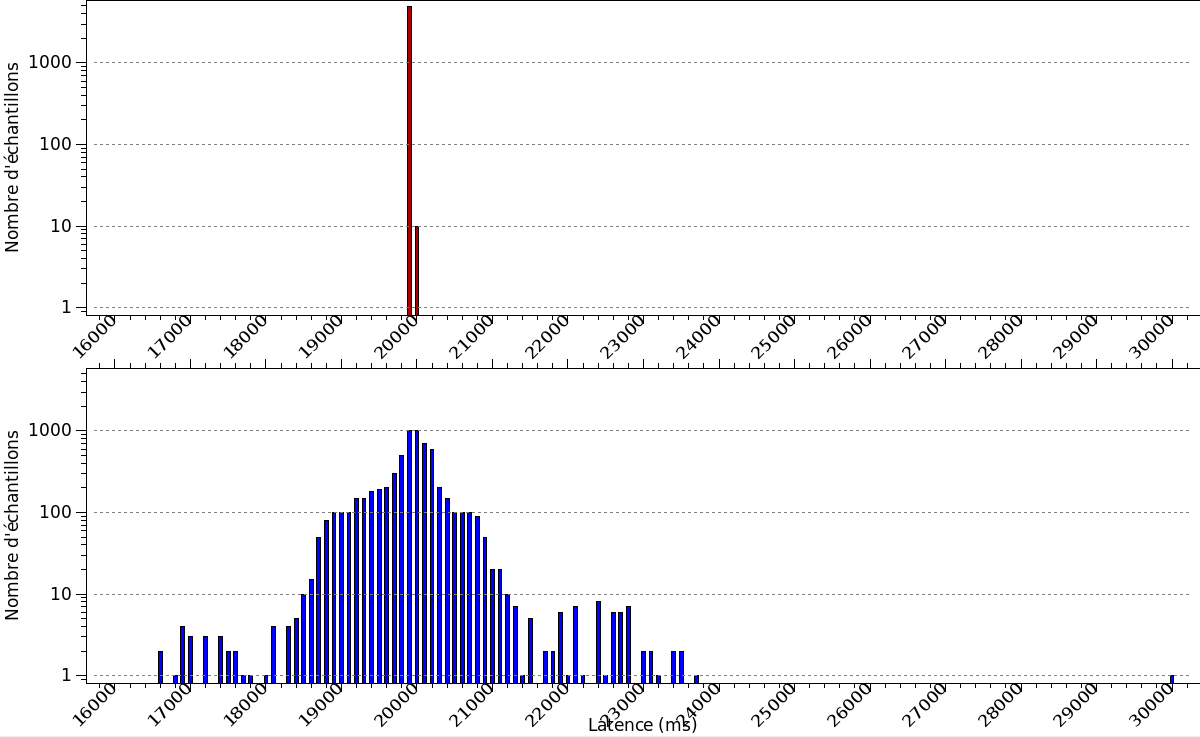
\includegraphics[width=10cm]{latency_2}
  \end{center}
\end{frame}

% Le temps de réponse ici est beaucoup mieux borné
% Schema des temps de réponses
\begin{frame}{Latence aux évènements}{Système temps réels}
  \begin{center}
    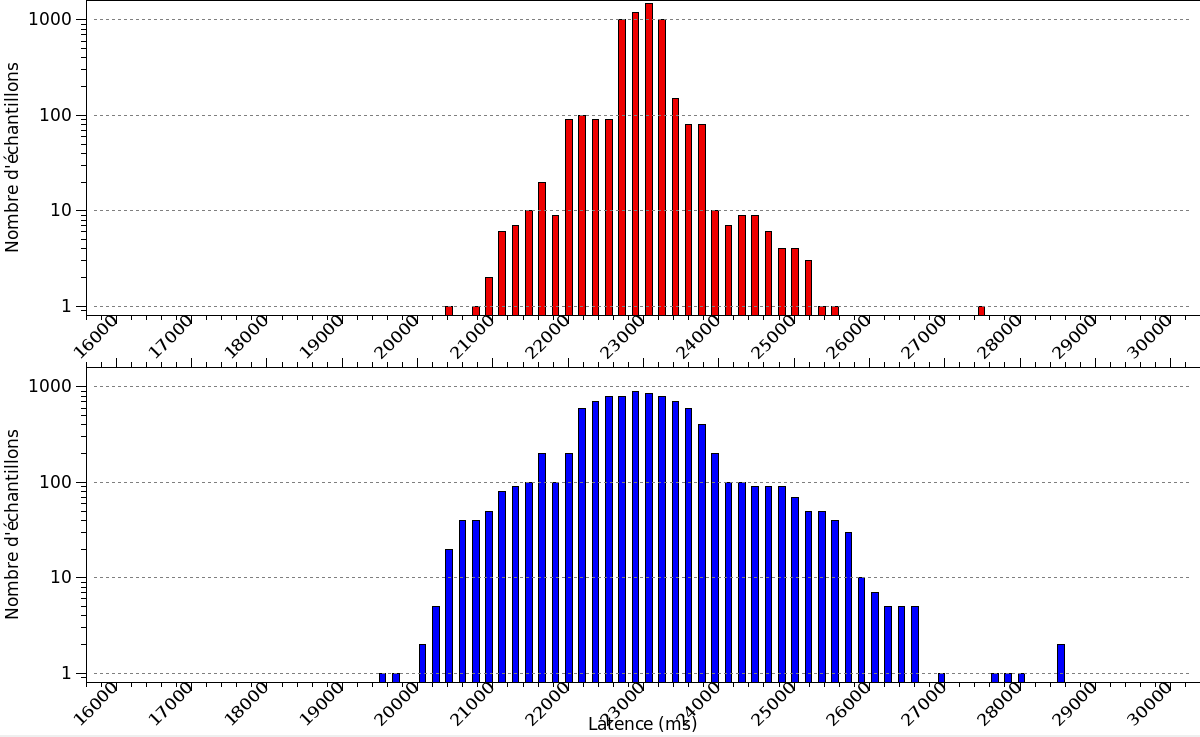
\includegraphics[width=10cm]{latency_1}
  \end{center}
\end{frame}
%     -> Taches RT << 100\%
%     ->  --> Algorithme d'ordonnancement secondaire (RM vs EDF)
%     -> Rendre cette formule assez simple pour être prédictible
%     %-> CAD limiter les effets des tache apériodique de priorité supérieure:
%        Interruptions, cache miss, changement de contexte, etc...
%     -> Présenter les diagramme normal va RT

\section{Systèmes Symétrique et asymétriques}

\begin{frame}{Systèmes symétriques}
\end{frame} 

\begin{frame}{Systèmes asymétriques}
\end{frame} 

\section{Low-latency}

\begin{frame}{Noyau low latency}{Problème du noyau normal} % 10min
 Un seul contexte noyau pour tout le monde
 \begin{itemize}
  \item Pas possible de préempter le système
  \item Personne ne peut prendre la main lorsqu'un processus est dans un syscall
  \item Équivalent d'une ressource partagée par tout les processus
  \item Possible de créer une gigantesque inversion de priorité
 \end{itemize}
\end{frame}

\begin{frame}{Noyau low latency}{Implémentation} % 10min
 \begin{itemize}
  \item Difficile de gérer les différents contextes noyau
  \item[$\to$] Noyau réentrant (= thread-safe)
  \item Gestion des interruption assez complexe
  \item Overhead assez important
 \end{itemize}
\end{frame}
%         -> Explique le problème des contexte noyaux
%         -> Définition de "Réentrant" (thread-safe)

\begin{frame}{Noyau low latency}{Résultats} % 5min
 \begin{itemize}
   \item Patch low-latency mergé dans le mainstream avec le noyau 2.6 (\texttt{CONFIG\_PREEMPT})
   \item Latences maximum de l'ordre de 300µs (chiffres de l'époque)
 \end{itemize}
\end{frame}
%      -> Patch low-latency, mergé dans le mainstream avec le noyau 2.6 (CONFIG\_PREEMPT)
%      -> A l'époque, on obtenait des latence max de l'ordre de 300µs

\section{Hyperviseurs} % (30min)

\begin{frame}{Hyperviseur}
  \begin{itemize}
    \item Noyau low latency encore problèmatique pour les interruptions
    \item Beaucoup d'interruptions $\to$ latence
    \item Hyperviseur
  \end{itemize}
\end{frame}
%      -> Utilisation d'un hyperviseur
%      -> Shéma RTLinux et ADEOS

% \begin{frame}{Temps réel}{Micro Kernel}
%   \includegraphics[height=6cm]{RT-microKernel.png}
% \end{frame}
% 
% \begin{frame}{Temps réel}{Nano Kernel}
%   \includegraphics[height=6cm]{RT-nanoKernel.png}
% \end{frame}
\begin{frame}{Temps réel}{Nano Kernel}
  \begin{center}
    \begin{tikzpicture}[scale=1.2]
      \draw[font=\small]
        node[size1, ccyan]   at (1, 2) {Tache temps réel}
        node[size1, ccyan]   at (3, 2) {Tache temps réel}
        node[size1, corange] at (5, 3) {Application}
        node[size1, corange] at (7, 3) {Application}
        node[size2, cred]    at (6, 2) {Noyau (non temps réel)}
        node[size4, cpurple] at (4, 1) {Hyperviseur}
        node[size4, cgreen]  at (4, 0) {Matériel};
    \end{tikzpicture}
  \end{center}
\end{frame}

\begin{frame}[fagile]{Hyperviseur}
  \begin{itemize}
   \item Possibilité de préempter le noyau sans patch low-latency
   \item Possibilité de differer les interruptions
   \item Possibilité d'ignorer les interruptions dans les sections temps réelles
   \item Performances excellentes (< 20µs)
   \item Technique non spécifique à Linux
   \item Peu de code en mode temps réelles
   \item[$\to$] Certifiable

   \item Fonctionne au dessus du noyau
   \item Comportement des interruptions à modifier
   \item Communication entre les tâches temps réelles et le reste
   \item[$\to$] Nécessite de patcher le noyau
   
   \item RTLinux, RTAI et Adeos (\texttt{http://download.gna.org/adeos/patches/}, \texttt{git://git.xenomai.org/ipipe-gch.git}) (Xenomai)
  \end{itemize}
\end{frame}

\begin{frame}{Hyperviseur}{Adeos}
  \begin{itemize}
    \item Fork de RTAI
    \item API utilisateur assurée par Xenomai
    \begin{itemize}
      \item Skins 
      \item[$\to$] Possibilité de faire fonctionner une application développée pour vxWorks
% Parler de vxWorks: Référence dans le domaine des OS RT Posix, OS des sondes Martiennes
      \item Skin native consistante
      \item Beaucoup mieux que Posix (de plus, il existe une skin Posix)
      \item \texttt{www.xenomai.org/documentation/xenomai-head/html/api}
    \end{itemize}
  \end{itemize}
\end{frame}
%      -> API utilisateur assurée par Xenomai
%         -> Skin, possibilité de faire fonctionner une application faite pour vxWorks
%         -> Skin native consistante
%         -> Beaucoup mieux que Posix (de plus, il existe une skin Posix)

% TP Interuptions avec Xenomai
% Mettre en place l'interruption RTC (8) voir Doucmentation/rtc.txt
\section{RT-préempt} % (30min)

\begin{frame}{RT-preempt} % (15min)
  Gestion des interruption dans des threads
%     -> Rappeller vous de nos spin_lock
  \begin{itemize}
    \item Permet de préempter les interruptions
    \item[$\to$] Moins de latence des taches
    \item Permet d'ordonnancer les interruption
    \item[$\to$] Permet de se passer de la désactivation des interruptions
    \item[$\to$] Permet de remplacer les spin lock par des mutex
    \item[$\to$] Moins de latence des interruptions
  \end{itemize}
\end{frame}

\begin{frame}{RT-preempt} 
  \begin{center}
    \begin{tikzpicture}[scale=1.2]
      \draw[font=\small]
        node[size2, corange]    at (6, 2) {Application}
        node[size2, corange]    at (2, 2) { } 
        node[size1]             at (3, 2) {Application}
        node[size1, ccyan, scale=0.9] at (1, 2) {Tache temps réel}
        node[size4, cred]       at (4, 1) { } 
        node[size3]             at (4, 1) {Noyau}
        node[size1, cpurple, scale=0.9] at (1, 1) {Tache temps réel}
        node[size4, cgreen]     at (4, 0) {Matériel};
    \end{tikzpicture}
  \end{center}
\end{frame}

\begin{frame}{RT-preempt}
 \begin{itemize}
  \item Patch RT (Patchs: \texttt{http://www.kernel.org/pub/linux/kernel/projects/rt/}, Git: \texttt{git://git.kernel.org/pub/scm/linux/kernel/git/rostedt/linux-2.6-rt.git})
  \item Implémentation assez complexe
  \item[$\to$] Non portable
  \item Performance très bonnes (~20µs)
 \end{itemize}
\end{frame}
%     -> Gère les interruption dans des thread
%     -> /!\ Pas portable partout
%     -> Implémentation assez tordue (c'est un cinglé qui a fait ca).
%     -> PatchRT


\end{document}

%%% Local Variables: 
%%% mode: latex
%%% TeX-master: t
%%% End: 
